\documentclass[conference]{IEEEtran}
\IEEEoverridecommandlockouts
% The preceding line is only needed to identify funding in the first footnote. If that is unneeded, please comment it out.
\usepackage{cite}
\usepackage{amsmath,amssymb,amsfonts}
\usepackage{algorithmic}
\usepackage{graphicx}
\usepackage{textcomp}
\usepackage{xcolor}
\usepackage{colortbl} % For colored table cells
\usepackage{booktabs} % For better tables
\usepackage{multirow} % For multirow cells in tables
\usepackage{url}      % For URLs
\usepackage{hyperref} % For clickable links (optional)
\usepackage{float}
\usepackage{subcaption}
\usepackage{booktabs}
\usepackage{threeparttable}
\usepackage{tabularx}
\usepackage{caption}
\def\BibTeX{{\rm B\kern-.05em{\sc i\kern-.025em b}\kern-.08em
    T\kern-.1667em\lower.7ex\hbox{E}\kern-.125emX}}

% Define colors for comments or notes (optional)
\usepackage{xcolor}
\newcommand{\todo}[1]{\textcolor{purple}{[TODO: #1]}}
\newcommand{\note}[1]{\textcolor{teal}{[Note: #1]}}


\begin{document}

\title{Comparative Analysis of Lion and AdamW Optimizers for Cross-Encoder Reranking with MiniLM, GTE, and ModernBERT}

% --- Author Information ---
% Use \and to separate authors if more than one
\author{\IEEEauthorblockN{Shahil Kumar}
\IEEEauthorblockA{\textit{IT} \\ 
\textit{IIIT Allahabad}\\
Prayagraj, India \\
mml2023008@iiita.ac.in}
\and % Uncomment and repeat for additional authors
\IEEEauthorblockN{Author 2 Name}
\IEEEauthorblockA{\textit{Department} \\
\textit{Institution}\\
City, Country \\
email address}
}
% --- End Author Information ---

\maketitle

\begin{abstract}
Modern information retrieval systems often employ a two-stage pipeline consisting of an efficient initial retrieval stage followed by a more computationally intensive reranking stage. Cross-encoder models have demonstrated state-of-the-art effectiveness for the reranking task due to their ability to perform deep, contextualized analysis of query-document pairs. The choice of optimizer during the fine-tuning phase can significantly impact the final performance and training efficiency of these models. This paper investigates the impact of using the recently proposed Lion optimizer compared to the widely used AdamW optimizer for fine-tuning cross-encoder rerankers. We fine-tune three distinct transformer models, `microsoft/MiniLM-L12-H384-uncased`, `Alibaba-NLP/gte-multilingual-base`, and `answerdotai/ModernBERT-base`, on the MS MARCO passage ranking dataset using both optimizers. Notably, GTE and ModernBERT support longer context lengths (8192 tokens). The effectiveness of the resulting models is evaluated on the TREC 2019 Deep Learning Track passage ranking task and the MS MARCO development set (for MRR@10). Our experiments, facilitated by the Modal cloud computing platform for GPU resource management, show comparative results across three training epochs. ModernBERT trained with Lion achieved the highest NDCG@10 (0.7225) and MAP (0.5121) on TREC DL 2019, while MiniLM trained with Lion achieved the highest MRR@10 (0.5988) on MS MARCO dev. We analyze the performance trends based on standard IR metrics, providing insights into the relative effectiveness of Lion versus AdamW for different model architectures and training configurations in the context of passage reranking.
\end{abstract}

\begin{IEEEkeywords}
Information Retrieval, Cross-Encoder, Reranking, Optimizer, Lion Optimizer, AdamW, TREC Deep Learning, MS MARCO, Sentence Transformers, ModernBERT, Long Context, Modal.
\end{IEEEkeywords}

\section{Introduction}
Information Retrieval (IR) systems aim to satisfy a user's information need, often expressed as a textual query, by returning a ranked list of relevant documents from a large collection. A common and effective architecture for modern search systems is the two-stage retrieve-and-rerank pipeline \cite{hu2019retrievereadrerankendtoend}. The first stage employs computationally efficient methods, such as BM25 \cite{robertson2009probabilistic} or dense vector retrieval \cite{karpukhin2020dense}, to quickly retrieve a candidate set of documents (typically hundreds or thousands) from the entire collection. The second stage then applies a more sophisticated and computationally expensive reranking model to reorder this smaller candidate set, aiming for higher precision at the top ranks.

Cross-encoder models, typically based on transformer architectures like BERT \cite{devlin2019bert}, have emerged as state-of-the-art rerankers \cite{nogueira2020passagererankingbert, Nogueira2020Document}. Unlike bi-encoder models that encode queries and documents independently, cross-encoders process the query and a candidate document simultaneously (e.g., `[CLS] query [SEP] document [SEP]`). This allows for deep, token-level interaction modeling, leading to superior relevance estimation accuracy, albeit at a higher computational cost suitable only for the second stage. Some models like GTE \cite{li2023towards} and ModernBERT \cite{modernbert} support significantly longer input sequences (e.g., 8192 tokens), potentially benefiting the processing of longer passages or documents compared to models with shorter context windows like MiniLM \cite{wang2020minilm}.

Fine-tuning these large transformer models effectively is crucial. The choice of optimizer plays a key role in navigating the complex loss landscape and achieving optimal performance. Adam \cite{kingma2017adam} and its variant AdamW \cite{loshchilov2019decoupled} are widely used and generally effective optimizers for training deep neural networks. Recently, the Lion (Evo\textbf{L}ved S\textbf{i}gn M\textbf{o}me\textbf{n}tum) optimizer \cite{chen2023symbolic} was proposed, derived through symbolic mathematics and program search. It claims improved performance and memory efficiency compared to AdamW on various tasks, particularly image classification and vision-language models.

In this work, we investigate the applicability and effectiveness of the Lion optimizer for fine-tuning cross-encoder models specifically for the task of passage reranking in information retrieval. We compare its performance against the standard AdamW optimizer across three different base models with varying characteristics. Our contributions are:
\begin{itemize}
    \item We fine-tune three distinct transformer-based cross-encoder models (`microsoft/MiniLM-L12-H384-uncased`, `Alibaba-NLP/gte-multilingual-base`, and `answerdotai/ModernBERT-base`) on the large-scale MS MARCO passage dataset \cite{DBLP:journals/corr/NguyenRSGTMD16} using both Lion and AdamW optimizers.
    \item We utilize different training configurations optimized for specific models, including a lower learning rate (2e-6) and a Cosine Annealing scheduler for ModernBERT, contrasting with a higher rate (2e-5) and no scheduler for MiniLM and GTE.
    \item We evaluate the performance of the fine-tuned models across three training epochs on the TREC 2019 Deep Learning (DL) Track \cite{craswell2020overview} benchmark and the MS MARCO development set \cite{DBLP:journals/corr/NguyenRSGTMD16}.
    \item We provide a comparative analysis of the optimizers' impact on reranking effectiveness using standard IR metrics (NDCG@10, MAP, MRR@10, Recall@10, R-Prec, P@10).
    \item We utilize the Modal cloud platform \cite{modal_labs} for efficient GPU resource management (NVIDIA A100-80GB) and reproducible experimentation.
\end{itemize}
The rest of the paper is organized as follows: Section \ref{sec:related_work} discusses related work. Section \ref{sec:methodology} details the models, optimizers, and training approach. Section \ref{sec:experimental_setup} describes the experimental setup, datasets, and evaluation protocol. Section \ref{sec:results} presents and discusses the results. Finally, Section \ref{sec:conclusion} concludes the paper and suggests future work.

\section{Related Work}
\label{sec:related_work}

\subsection{Cross-Encoder Reranking}
The use of BERT-based models for document reranking was popularized by Nogueira et al. \cite{nogueira2020passagererankingbert, Nogueira2020Document}. They demonstrated that fine-tuning BERT as a cross-encoder on relevance labels (like those from MS MARCO) significantly outperforms traditional IR models and even bi-encoder approaches for reranking tasks. Subsequent work explored various transformer architectures \cite{Lin2021PretrainedTF}, training strategies \cite{gao2021complementing}, and efficiency improvements \cite{hofstatter2020improving}. Models like MiniLM \cite{wang2020minilm} offer a balance between effectiveness and efficiency through knowledge distillation. Multilingual models like GTE \cite{li2023towards} (General Text Embeddings) provide strong performance across various text tasks, including retrieval, and can be adapted for cross-encoding, supporting longer context lengths. Recently, models like ModernBERT \cite{modernbert} have incorporated architectural improvements such as Rotary Positional Embeddings (RoPE) \cite{su2023roformerenhancedtransformerrotary} and Flash Attention \cite{dao2022flashattentionfastmemoryefficientexact} to handle even longer sequences (up to 8192 tokens) efficiently and effectively. The `sentence-transformers` library \cite{reimers2019sentence} provides a convenient framework for training and using both bi-encoders and cross-encoders.

\subsection{Optimizers for Deep Learning}
Stochastic Gradient Descent (SGD) with momentum remains a fundamental optimizer, but adaptive learning rate methods like AdaGrad \cite{duchi2011adaptive}, RMSprop \cite{tieleman2012lecture}, and Adam \cite{kingma2017adam} often lead to faster convergence in practice for deep learning models. Adam combines momentum with adaptive scaling of learning rates based on estimates of first and second moments of the gradients. AdamW \cite{loshchilov2019decoupled} improves upon Adam by decoupling the weight decay regularization from the adaptive learning rate mechanism, often leading to better generalization. The Lion optimizer \cite{chen2023symbolic} takes a different approach, using only momentum tracking and a sign operation on the update, resulting in a simpler update rule (`update = sign(momentum) * lr`) and potentially requiring less memory due to not storing second moment estimates. Its effectiveness relative to AdamW has been shown primarily in vision and vision-language tasks, motivating its evaluation in the NLP/IR domain.

\subsection{Evaluation Benchmarks}
The MS MARCO (Microsoft MAchine Reading COmprehension) dataset \cite{DBLP:journals/corr/NguyenRSGTMD16, DBLP:journals/corr/NguyenRSGTMD16} has become a standard benchmark for training and evaluating deep learning models for passage retrieval and reranking. It contains real user queries from Bing and human-judged relevant passages. The TREC Deep Learning (DL) Tracks \cite{craswell2020overview, craswell2021overview} provide challenging test collections built upon MS MARCO, using queries with sparse relevance judgments derived from pooling top results from various participating systems. We use the TREC DL 2019 passage ranking dataset, a standard benchmark for evaluating reranking effectiveness. Evaluation is typically performed using tools like `trec\_eval` \cite{trec_eval_github}, which calculates various standard IR metrics. We specifically use the MS MARCO passage dataset's development split for evaluating MRR@10, providing a complementary perspective on a larger query set.

\section{Methodology}
\label{sec:methodology}

\subsection{Cross-Encoder Architecture}
A cross-encoder model takes a query $q$ and a document $d$ as input, typically concatenating them with special tokens: `[CLS] q [SEP] d [SEP]`. This combined sequence is fed into a transformer model (e.g., MiniLM, GTE, ModernBERT). The output representation corresponding to the `[CLS]` token is then passed through a linear layer followed by a sigmoid activation to predict a relevance score $s(q, d) \in [0, 1]$. During inference for reranking, this score is computed for all candidate documents retrieved in the first stage, and the documents are re-sorted based on these scores. An overview of the architecture is shown in Fig. \ref{fig:cross_encoder_arch}.

\begin{figure}[htbp]
\centering
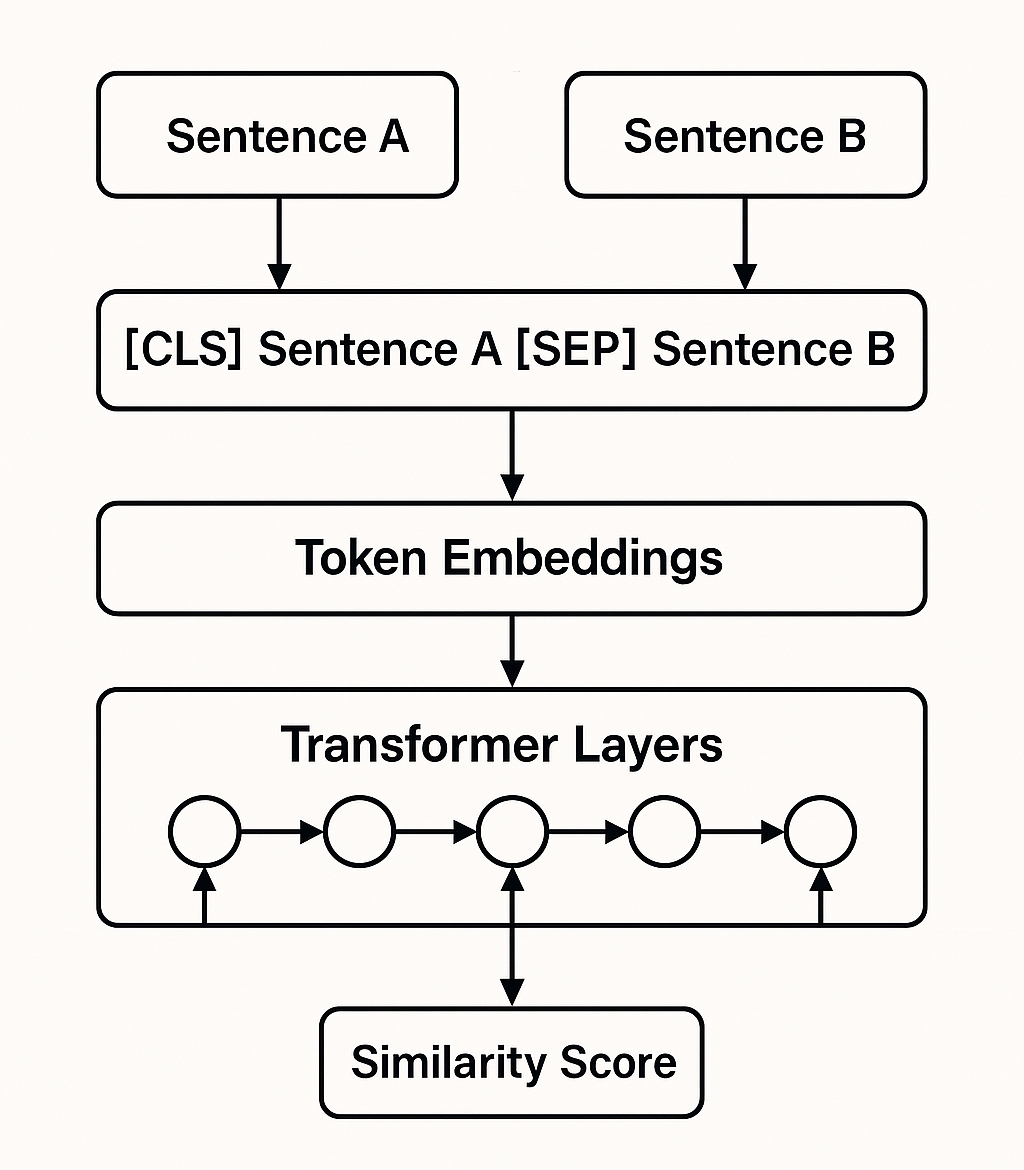
\includegraphics[width=0.9\linewidth]{figures/cross_encoder_archi.png}
\caption{General Cross-Encoder Architecture for Reranking.}
\label{fig:cross_encoder_arch}
\end{figure}


\subsection{Base Models}
We experiment with three transformer base models from Hugging Face \cite{wolf2020transformers}:
\begin{itemize}
    \item \textbf{`microsoft/MiniLM-L12-H384-uncased` \cite{wang2020minilm}:} A distilled version of BERT, designed to be smaller (12 layers, 384 hidden size) and faster while retaining significant performance. It has a standard context length, typically 512 tokens.
    \item \textbf{`Alibaba-NLP/gte-multilingual-base` \cite{li2023towards}:} Part of the General Text Embeddings (GTE) family, trained on a large, diverse multilingual corpus. While often used as a bi-encoder, its underlying transformer architecture can be effectively fine-tuned as a cross-encoder. This 'base' version supports a context length of 8192 tokens.
    \item \textbf{`answerdotai/ModernBERT-base` \cite{modernbert}:} A state-of-the-art encoder-only transformer incorporating architectural enhancements like Rotary Positional Embeddings (RoPE) \cite{su2023roformerenhancedtransformerrotary} for effective long context handling (up to 8192 tokens), Flash Attention \cite{dao2022flashattentionfastmemoryefficientexact} for speed and memory efficiency, and GeGLU activation functions \cite{shazeer2020gluvariantsimprovetransformer}. It was trained on 2 trillion tokens and demonstrates strong performance on various tasks.
\end{itemize}

\subsection{Training}
We fine-tune the cross-encoders using the MS MARCO passage ranking triplets dataset \cite{DBLP:journals/corr/NguyenRSGTMD16}, as processed by `sentence-transformers` \cite{reimers2019sentence}. The original dataset contains tuples of (query, positive passage, negative passage). We convert this into pairs `(query, positive\_passage)` with label 1 and `(query, negative\_passage)` with label 0. We train on approximately 2 million such pairs.
The training objective is to minimize the Binary Cross-Entropy (BCE) loss between the predicted relevance score $\hat{y}$ (output of the sigmoid function) and the true label $y$ (0 or 1). The BCE loss is defined as:
\[ \mathcal{L}_{BCE} = - [y \log(\hat{y}) + (1 - y) \log(1 - \hat{y})] \]

% \subsection{Optimizers}
% We compare two optimizers using specified parameters:
% \begin{itemize}
%     \item \textbf{AdamW \cite{loshchilov2019decoupled}:} Implemented via `torch.optim.AdamW`. We use a weight decay of 0.01. The learning rate varies by model (see Section \ref{sec:experimental_setup}).
%     \item \textbf{Lion \cite{chen2023symbolic}:} Implemented via a PyTorch implementation based on the original paper. We use the default betas $\beta_1 = 0.9$, $\beta_2 = 0.99$, and a weight decay of 0.01. The learning rate varies by model. The core update rule relies on the sign of the momentum:
% \begin{align*}
% \text{update}_t &\leftarrow \beta_1 m_{t-1} + (1 - \beta_1) g_t \\
% \theta_t &\leftarrow \theta_{t-1} - \eta \cdot \text{sign}(\beta_2 \text{update}_t + (1 - \beta_2) g_t) - \eta \lambda \theta_{t-1}
% \end{align*}
% \noindent where $g_t$ is the gradient, $m_t$ is the momentum, $\eta$ is the learning rate, $\beta_1, \beta_2$ are momentum coefficients, and $\lambda$ is the weight decay.
% \end{itemize}

\subsection{Optimizers}
We compare two optimizers using specified parameters:
\begin{itemize}
    \item \textbf{AdamW \cite{loshchilov2019decoupled}:} Implemented via \texttt{torch.optim.AdamW}. We use a weight decay of 0.01. The learning rate varies by model (see Section \ref{sec:experimental_setup}).
    \item \textbf{Lion \cite{chen2023symbolic}:} Implemented via a PyTorch implementation based on the original paper. We use the default betas $\beta_1 = 0.9$, $\beta_2 = 0.99$, and a weight decay of 0.01. The learning rate varies by model. The update rule is as follows:
    \begin{align*}
    c_t &= \beta_1 m_{t-1} + (1 - \beta_1) g_t \\
    \theta_t &= \theta_{t-1} - \eta \left( \text{sign}(c_t) + \lambda \theta_{t-1} \right) \\
    m_t &= \beta_2 m_{t-1} + (1 - \beta_2) g_t
    \end{align*}
    where $g_t$ is the gradient, $m_t$ is the momentum, $\eta$ is the learning rate, $\beta_1, \beta_2$ are momentum coefficients, and $\lambda$ is the weight decay.
\end{itemize}

\section{Experimental Setup}
\label{sec:experimental_setup}

\subsection{Datasets}
\begin{itemize}
    \item \textbf{Training:} We use the MS MARCO passage ranking triplets dataset \cite{DBLP:journals/corr/NguyenRSGTMD16}, processed into approximately 2 million query-passage pairs with binary labels using the `sentence-transformers` methodology.
    \item \textbf{Evaluation (Main):} We evaluate on the TREC 2019 Deep Learning Track passage ranking task \cite{craswell2020overview}, which contains 43 queries with graded relevance judgments (qrels).
    \item \textbf{Evaluation (MRR@10):} We evaluate Mean Reciprocal Rank at cutoff 10 (MRR@10) on the MS MARCO passage dataset's development split (available from Hugging Face Datasets \cite{DBLP:journals/corr/NguyenRSGTMD16}), containing a larger set of queries with binary relevance.
\end{itemize}

\subsection{Implementation Details}
\begin{itemize}
    \item \textbf{Framework:} We use `sentence-transformers` \cite{reimers2019sentence} (`CrossEncoder`) built on PyTorch \cite{paszke2019pytorchimperativestylehighperformance} and Hugging Face Transformers \cite{wolf2020transformers}.
    \item \textbf{Hyperparameters:} Key training parameters are:
        \begin{itemize}
            \item Batch Size: 64.
            \item Learning Rate:
                \begin{itemize}
                    \item 2e-5 for MiniLM and GTE (both optimizers).
                    \item 2e-6 for ModernBERT with Lion optimizer.
                    \item 2e-5 for ModernBERT with adamW optmizer.
                \end{itemize}
            \item Scheduler:
                \begin{itemize}
                    \item None for MiniLM and GTE.
                    \item CosineAnnealingLR Scheduler for ModernBERT, with `T\_max` set to the total number of training steps.
                \end{itemize}
            \item Optimizer Params:
                \begin{itemize}
                    \item AdamW: weight\_decay=0.01.
                    \item Lion: betas=(0.9, 0.99), weight\_decay=0.01.
                \end{itemize}
            \item Warmup Ratio: 0.1 (for LR scheduler if used)
            \item Epochs: 3
            \item Precision: BF16 enabled.
            \item Seed: 12 (for reproducibility).
            \item Dataloader Workers: 4.
        \end{itemize}
    \item \textbf{Infrastructure:} 
    \begin{itemize}
        \item Experiments were conducted using the Modal platform \cite{modal_labs}, leveraging NVIDIA A100-80GB GPUs. Modal managed the environment (CUDA, Python 3.11, libraries) and distributed training.

        \item Experiment tracking, visualization of training metrics (such as loss and learning rate, see Fig. \ref{fig:modernbert_training_plots}), and hyperparameter logging were managed using the Weights \& Biases (W\&B) platform \cite{wandb2020}.
    \end{itemize}

    \item \textbf{First-Stage Retrieval:} For TREC DL evaluation, we retrieve the top 1000 candidate passages per query using a standard BM25 baseline via Pyserini \cite{lin2021pyserini} on the `msmarco-v1-passage` index. The cross-encoders rerank this candidate set.
\end{itemize}

\subsection{Evaluation Protocol}
\begin{itemize}
    \item \textbf{Reranking:} Each fine-tuned cross-encoder model scores the top-1000 BM25 candidates for each TREC DL 2019 query. Passages are reranked based on these scores.
    \item \textbf{Metrics:} We use `trec\_eval` \cite{trec_eval_github} for TREC DL 2019 evaluation. We report:
        \begin{itemize}
            \item NDCG@10 (Normalized Discounted Cumulative Gain @10)
            \item MAP (Mean Average Precision)
            \item Recall@10 (Recall @10)
            \item R-Prec (R-Precision)
            \item P@10 (Precision @10)
        \end{itemize}
    For MRR@10, we evaluate on the MS MARCO development set.
    \item \textbf{Configurations Tested:} We evaluate each combination of base model and optimizer after each of the 3 training epochs:
        \begin{itemize}
            \item MiniLM + AdamW (Epochs 1, 2, 3)
            \item MiniLM + Lion (Epochs 1, 2, 3)
            \item GTE-multilingual-base + AdamW (Epochs 1, 2, 3)
            \item GTE-multilingual-base + Lion (Epochs 1, 2, 3)
            \item ModernBERT-base + AdamW (Epochs 1, 2, 3)
            \item ModernBERT-base + Lion (Epochs 1, 2, 3)
        \end{itemize}
\end{itemize}

\section{Results and Discussion}
\label{sec:results}
Table \ref{tab:main_results} presents the evaluation results for all configurations on the TREC 2019 Deep Learning Track (NDCG@10, MAP, Recall@10, R-Prec, P@10) and MS MARCO development set (MRR@10) after 1, 2, and 3 epochs of fine-tuning. Best results for each metric are highlighted.

\begin{table*}[htbp]
\centering
\caption{Evaluation Results on TREC-DL 2019 and MS-MARCO Dev Passage Ranking}
\label{tab:main_results}
\begin{tabular}{l l c c c c c c c}
\toprule
\textbf{Base Model} & \textbf{Optimizer} & \textbf{Epoch} & \textbf{NDCG@10} & \textbf{MAP} & \textbf{MRR@10} & \textbf{Recall@10} & \textbf{R-Prec} & \textbf{P@10} \\
\midrule
\multirow{3}{*}{MiniLM-L12-H384} & \multirow{3}{*}{AdamW}
    & 1 & 0.7008 & 0.4814 & 0.5828 & 0.1712 & 0.4899 & 0.8047 \\
    & & 2 & 0.7094 & 0.4891 & 0.5818 & 0.1715 & 0.5017 & 0.8093 \\
    & & 3 & 0.7127 & 0.4908 & 0.5826 & 0.1706 & 0.4962 & 0.8023 \\
\midrule
\multirow{3}{*}{MiniLM-L12-H384} & \multirow{3}{*}{Lion}
    & 1 & 0.7031 & 0.4858 & 0.5890 & 0.1698 & 0.4904 & 0.8070 \\
    & & 2 & 0.6916 & 0.4755 & 0.5942 & 0.1724 & 0.5041 & 0.8116 \\
    & & 3 & 0.6808 & 0.4706 & \cellcolor{yellow!50}\textbf{0.5988} & 0.1701 & 0.4923 & 0.8023 \\
\midrule
\multirow{3}{*}{GTE-multilingual-base} & \multirow{3}{*}{AdamW}
    & 1 & 0.7224 & 0.5005 & 0.5940 & 0.1733 & 0.4957 & 0.8140 \\
    & & 2 & 0.7203 & 0.4999 & 0.5942 & \cellcolor{yellow!50}\textbf{0.1733} & 0.5067 & 0.8163 \\
    & & 3 & 0.6902 & 0.4899 & 0.5972 & 0.1730 & 0.5069 & 0.8140 \\
\midrule
\multirow{3}{*}{GTE-multilingual-base} & \multirow{3}{*}{Lion}
    & 1 & 0.6785 & 0.4754 & 0.5854 & 0.1684 & 0.4849 & 0.7953 \\
    & & 2 & 0.6909 & 0.4921 & 0.5957 & 0.1721 & 0.5053 & 0.8140 \\
    & & 3 & 0.6904 & 0.4912 & 0.5931 & 0.1719 & 0.5041 & 0.8093 \\
\midrule
\multirow{3}{*}{Modern-BERT-base} & \multirow{3}{*}{AdamW}
    & 1 & 0.7105 & 0.5066 & 0.5865 & 0.1678 & 0.5161 & 0.8163 \\
    & & 2 & 0.6839 & 0.4893 & 0.5885 & 0.1634 & 0.4946 & 0.7814 \\
    & & 3 & 0.6959 & 0.4971 & 0.5916 & 0.1623 & 0.5116 & 0.7860 \\ % Corrected P@10 based on context
\midrule
\multirow{3}{*}{Modern-BERT-base} & \multirow{3}{*}{Lion}
    & 1 & 0.7142 & \cellcolor{yellow!50}\textbf{0.5121} & 0.5834 & 0.1689 & 0.5148 & 0.8163 \\
    & & 2 & \cellcolor{yellow!50}\textbf{0.7225} & 0.5115 & 0.5907 & 0.1732 & \cellcolor{yellow!50}\textbf{0.5183} & 0.8209 \\
    & & 3 & 0.7051 & 0.5020 & \cellcolor{yellow!50}\textbf{0.5988}* & 0.1722 & 0.5102 & \cellcolor{yellow!50}\textbf{0.8256} \\
\bottomrule
\end{tabular}
\vspace{1em}\\
\footnotesize{* MRR@10 is calculated on the MS MARCO v1.1 passage dataset development split. All other metrics are calculated on TREC DL 2019. Best result for each metric highlighted. (*Note: MiniLM+Lion also achieved 0.5988 MRR@10 at epoch 3, (see Appendix A for complete metrics).)}
\end{table*}

\subsection{Optimizer Performance Comparison}
We observe different interactions between the base models and the optimizers:

\begin{itemize}
    \item **MiniLM:** AdamW generally achieves higher peak performance on TREC DL 2019 metrics (NDCG@10: 0.7127 vs 0.7031; MAP: 0.4908 vs 0.4858), peaking at Epoch 3. Lion achieves the overall best MRR@10 on MS MARCO dev (0.5988 at Epoch 3), but its TREC performance peaks earlier (Epoch 1) and then declines. This suggests AdamW might be more stable over longer training for MiniLM on TREC, while Lion might converge faster or optimize differently for the MS MARCO distribution.
    \item **GTE:** AdamW clearly outperforms Lion for the GTE model across most metrics and epochs. GTE+AdamW achieves its best TREC performance (NDCG@10=0.7224, MAP=0.5005) early at Epoch 1 or 2, with performance degrading by Epoch 3. GTE+Lion shows weaker performance overall, peaking later (Epoch 2/3) but never reaching the levels of GTE+AdamW.
    \item **ModernBERT:** Lion significantly outperforms AdamW when training ModernBERT with the specific low learning rate (2e-6) and Cosine Annealing scheduler. ModernBERT+Lion achieves the overall best NDCG@10 (0.7225), MAP (0.5121), R-Prec (0.5183), and P@10 (0.8256) in our experiments. Its performance peaks around Epoch 2 for most TREC metrics. ModernBERT+AdamW, using the same LR and scheduler, performed notably worse, suggesting Lion interacts more favorably with this setup for this model.
\end{itemize}
These results indicate that the choice of optimizer interacts significantly with the base model architecture and the specific training hyperparameters (learning rate, scheduler). Lion showed particular strength with ModernBERT under its tailored training regime.

\subsection{Model Performance Comparison}
Comparing the best results achieved by each model (irrespective of optimizer epoch):

\begin{itemize}
    \item **ModernBERT (+Lion, E2/E1/E3):** Achieved the highest NDCG@10 (0.7225), MAP (0.5121), R-Prec (0.5183), and P@10 (0.8256) on TREC DL 2019, and tied for the best MRR@10 (0.5988) on MS MARCO dev. This suggests its advanced architecture and long context, combined with the Lion optimizer and specific training strategy, yield superior reranking quality.
    \item **GTE (+AdamW, E1/E2):** Achieved the next best performance, with NDCG@10 (0.7224) nearly matching ModernBERT+Lion, and achieving the best Recall@10 (0.1733). Its peak performance was reached earlier than ModernBERT's in terms of epochs.
    \item **MiniLM (+AdamW E3 / +Lion E3):** While performing competitively, MiniLM generally lagged behind GTE and ModernBERT on TREC metrics. However, MiniLM+Lion achieved the joint-highest MRR@10 (0.5988) on the MS MARCO dev set, indicating strong performance on that specific benchmark despite lower TREC scores compared to the larger models.
\end{itemize}
The results suggest that the larger models with longer context capabilities (GTE, ModernBERT) generally outperform MiniLM on the TREC DL 2019 task. ModernBERT, with its specific optimizations and training configuration using Lion, achieved the overall best effectiveness.

\subsection{Performance Trends Over Epochs and Training Dynamics}
Observing Table \ref{tab:main_results}, performance is not always monotonic with training epochs.
\begin{itemize}
    \item GTE+AdamW peaks early (Epoch 1 or 2) and then degrades.
    \item MiniLM+AdamW shows more gradual improvement or stability up to Epoch 3.
    \item MiniLM+Lion peaks early on TREC (Epoch 1) but late on MS MARCO MRR (Epoch 3).
    \item ModernBERT+Lion mostly peaks around Epoch 2.
    \item ModernBERT+AdamW performance is less consistent, potentially indicating suboptimal interaction with the LR/scheduler setup.
\end{itemize}
This highlights the importance of evaluating at multiple checkpoints. Additionally, analysis of training/evaluation loss curves, learning rate schedules, and gradient norms (Fig. \ref{fig:modernbert_training_plots}) for ModernBERT provides further insight into the training dynamics, showing convergence patterns under the Cosine Annealing schedule with both optimizers.

\begin{figure*}[htbp]
\centering

\begin{subfigure}[b]{0.45\textwidth}
    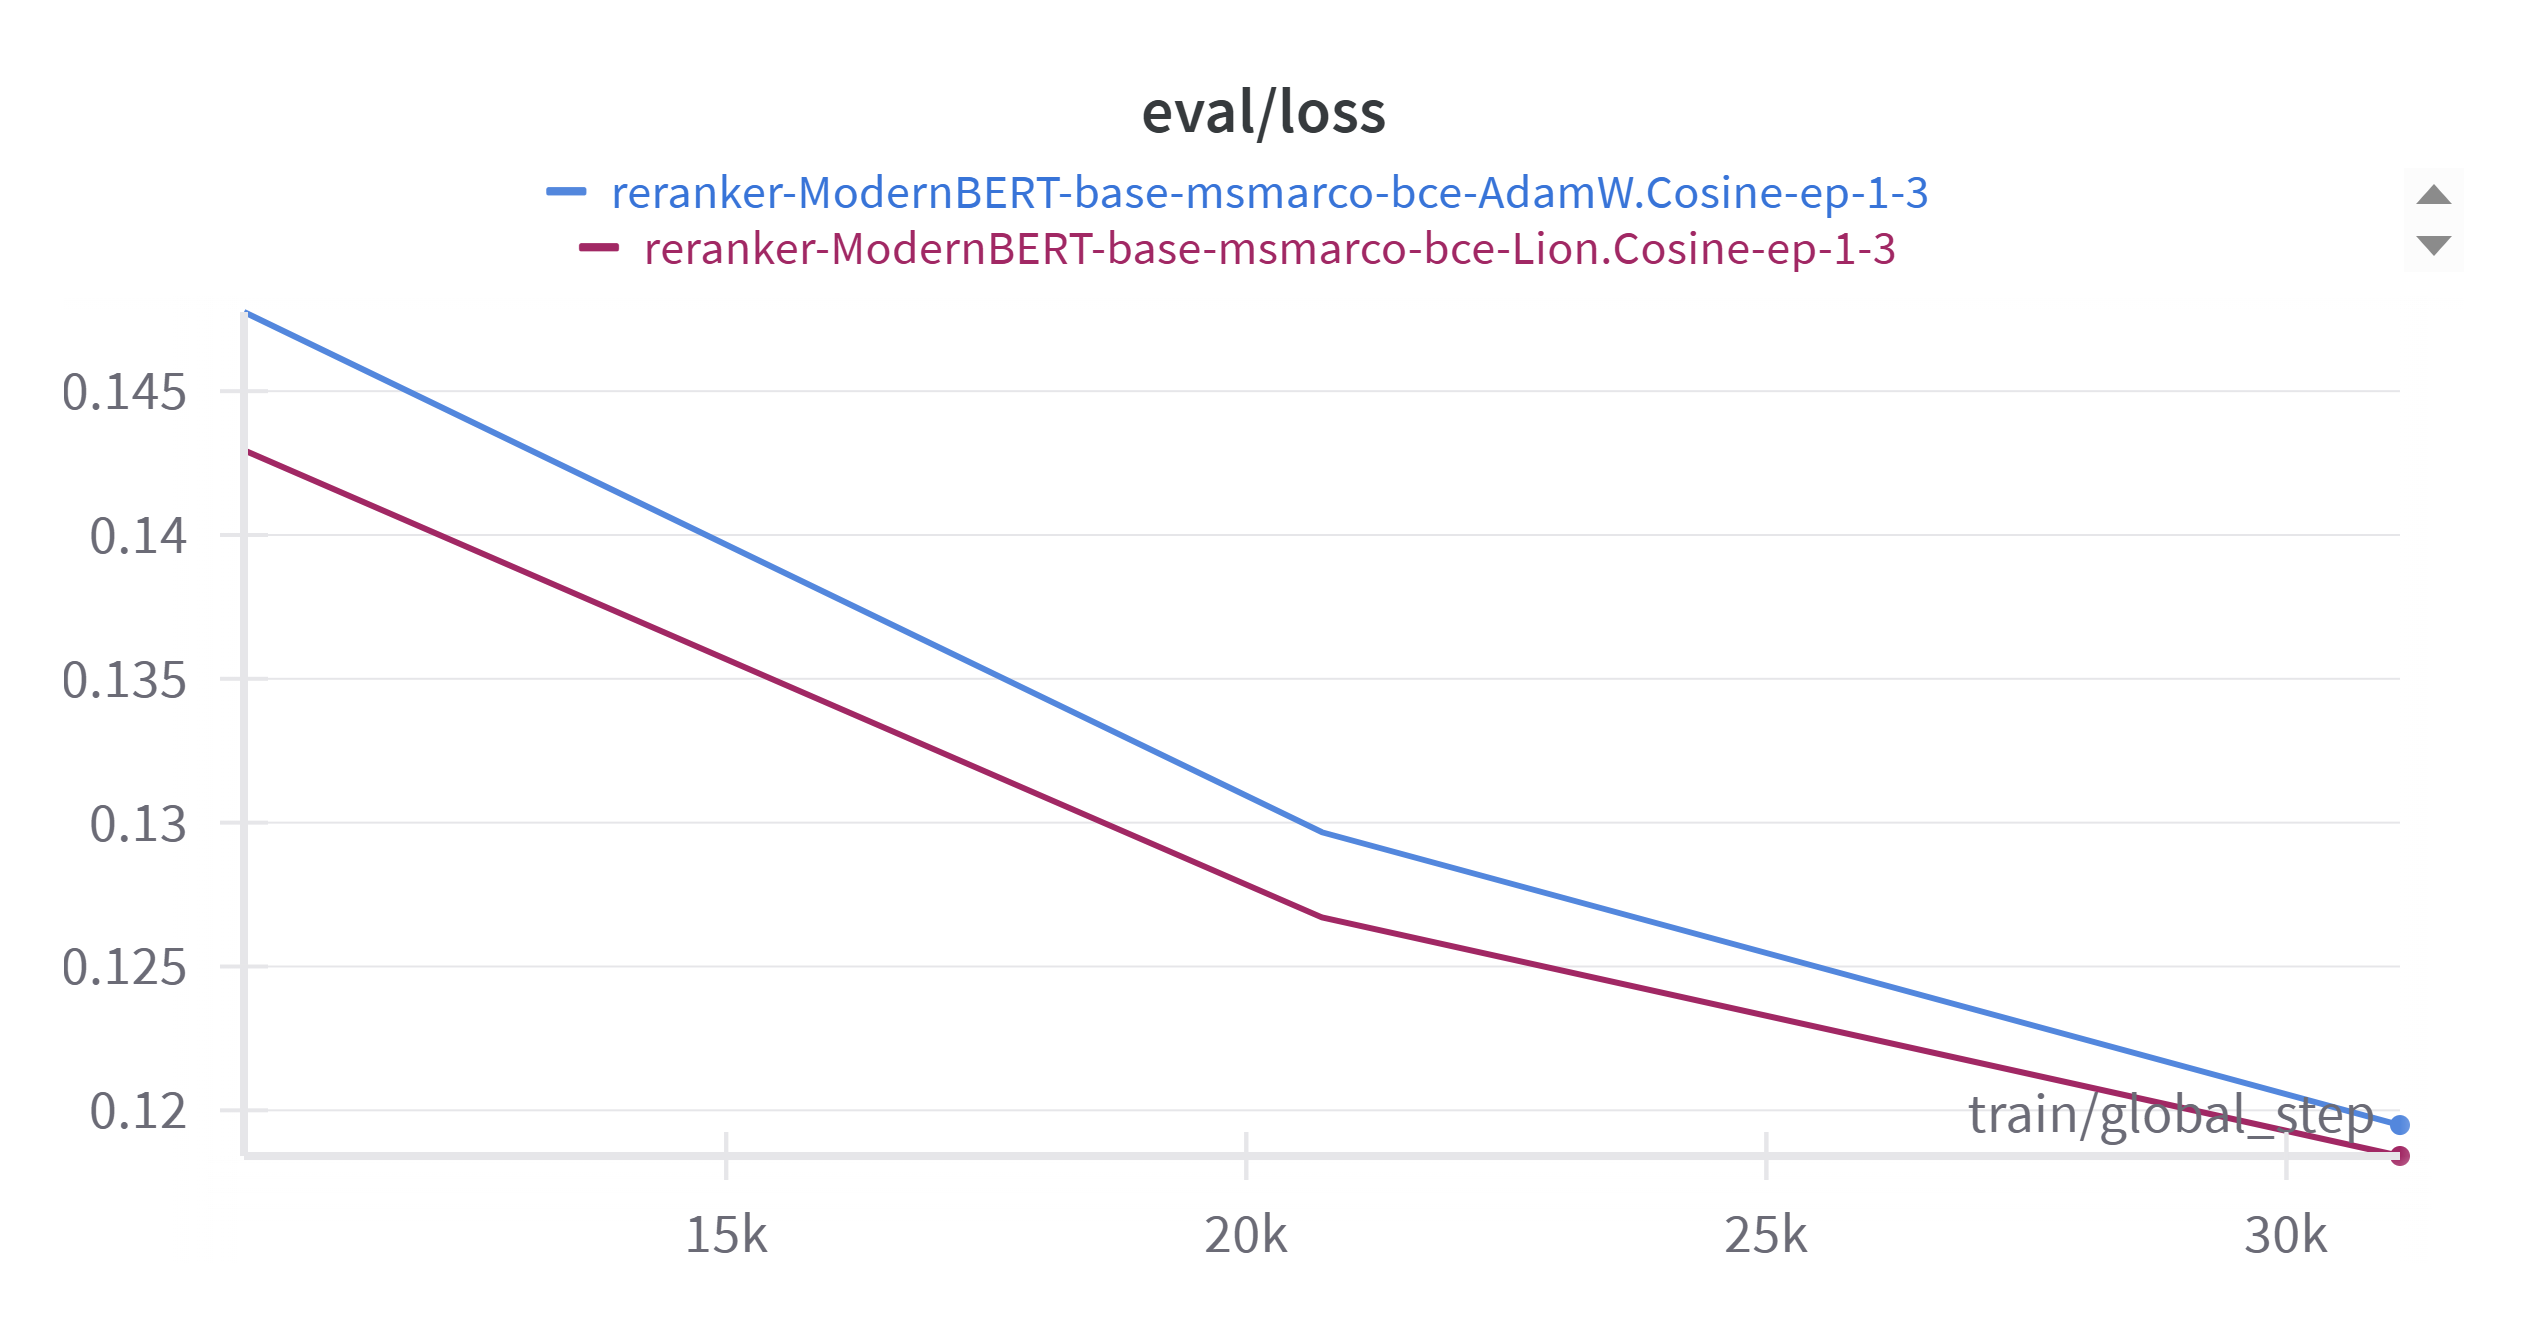
\includegraphics[width=\linewidth]{figures/modernBERT-Lion-AdamW-eval_loss.png}
    \caption{Eval Loss}
    \label{fig:modernbert_eval_loss}
\end{subfigure}
\hfill
\begin{subfigure}[b]{0.45\textwidth}
    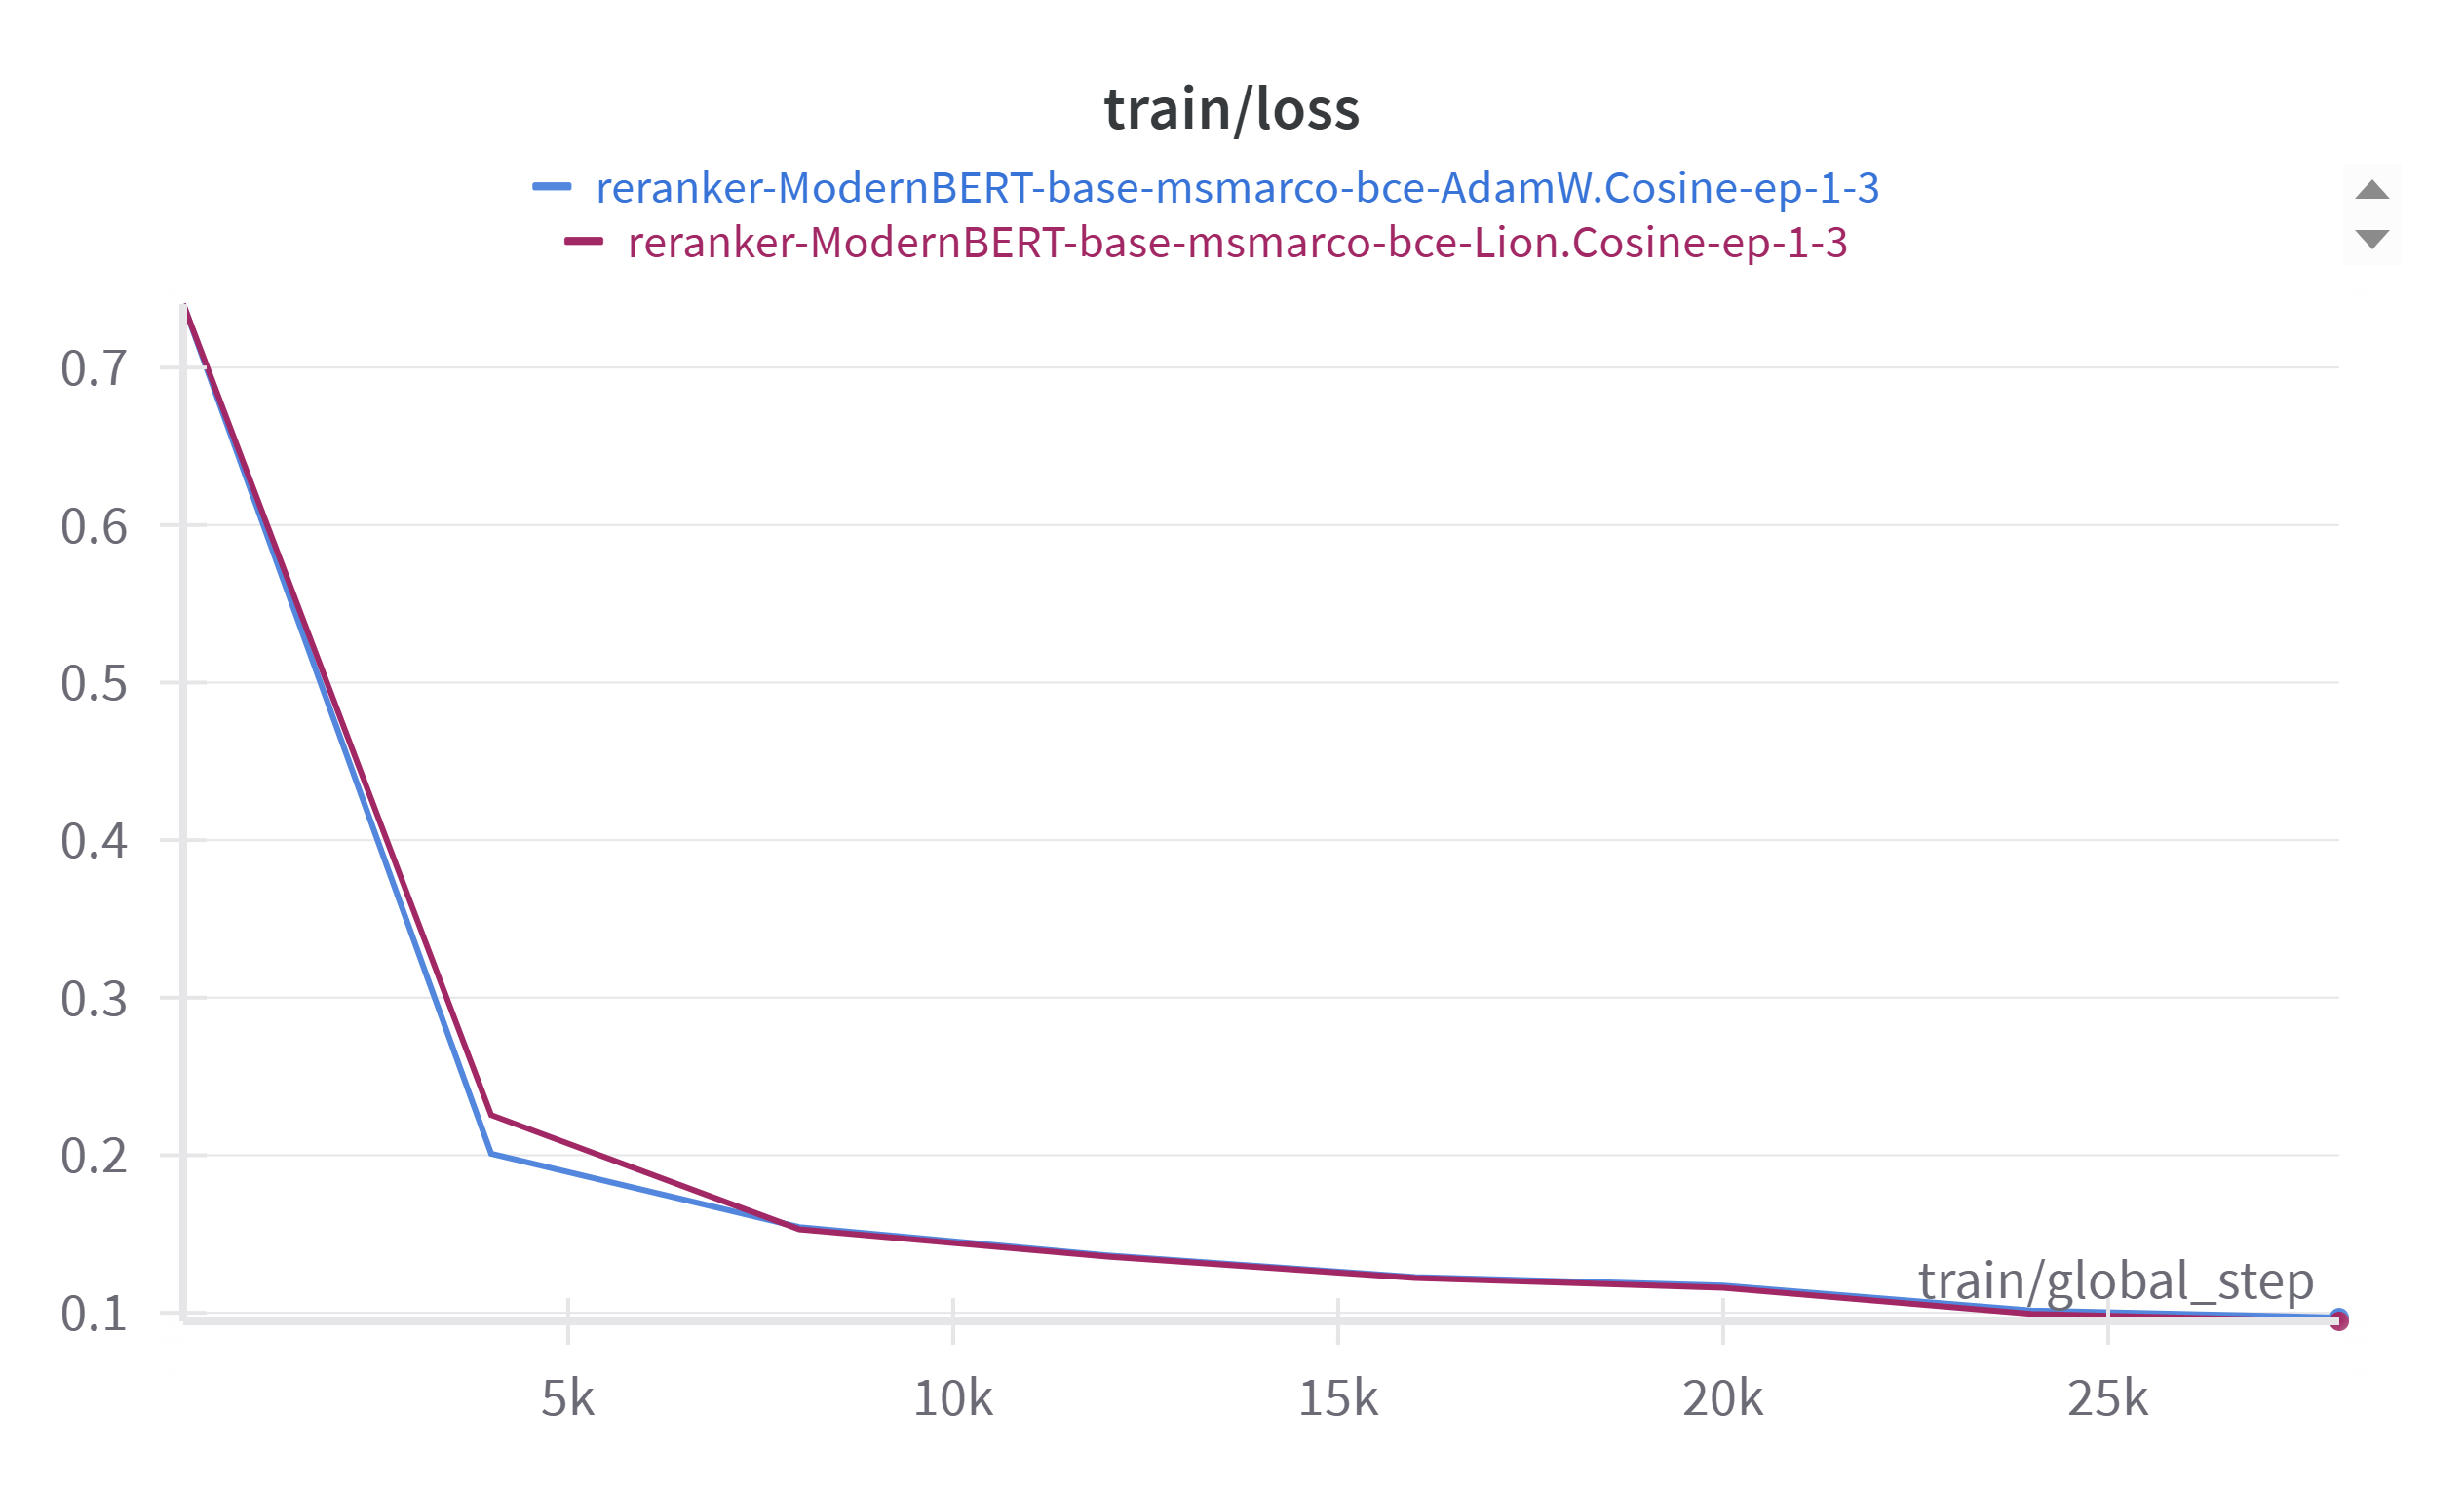
\includegraphics[width=\linewidth]{figures/modernBERT-Lion-adamW-train_loss.png}
    \caption{Train Loss}
    \label{fig:modernbert_train_loss}
\end{subfigure}

\vspace{0.5cm}

\begin{subfigure}[b]{0.45\textwidth}
    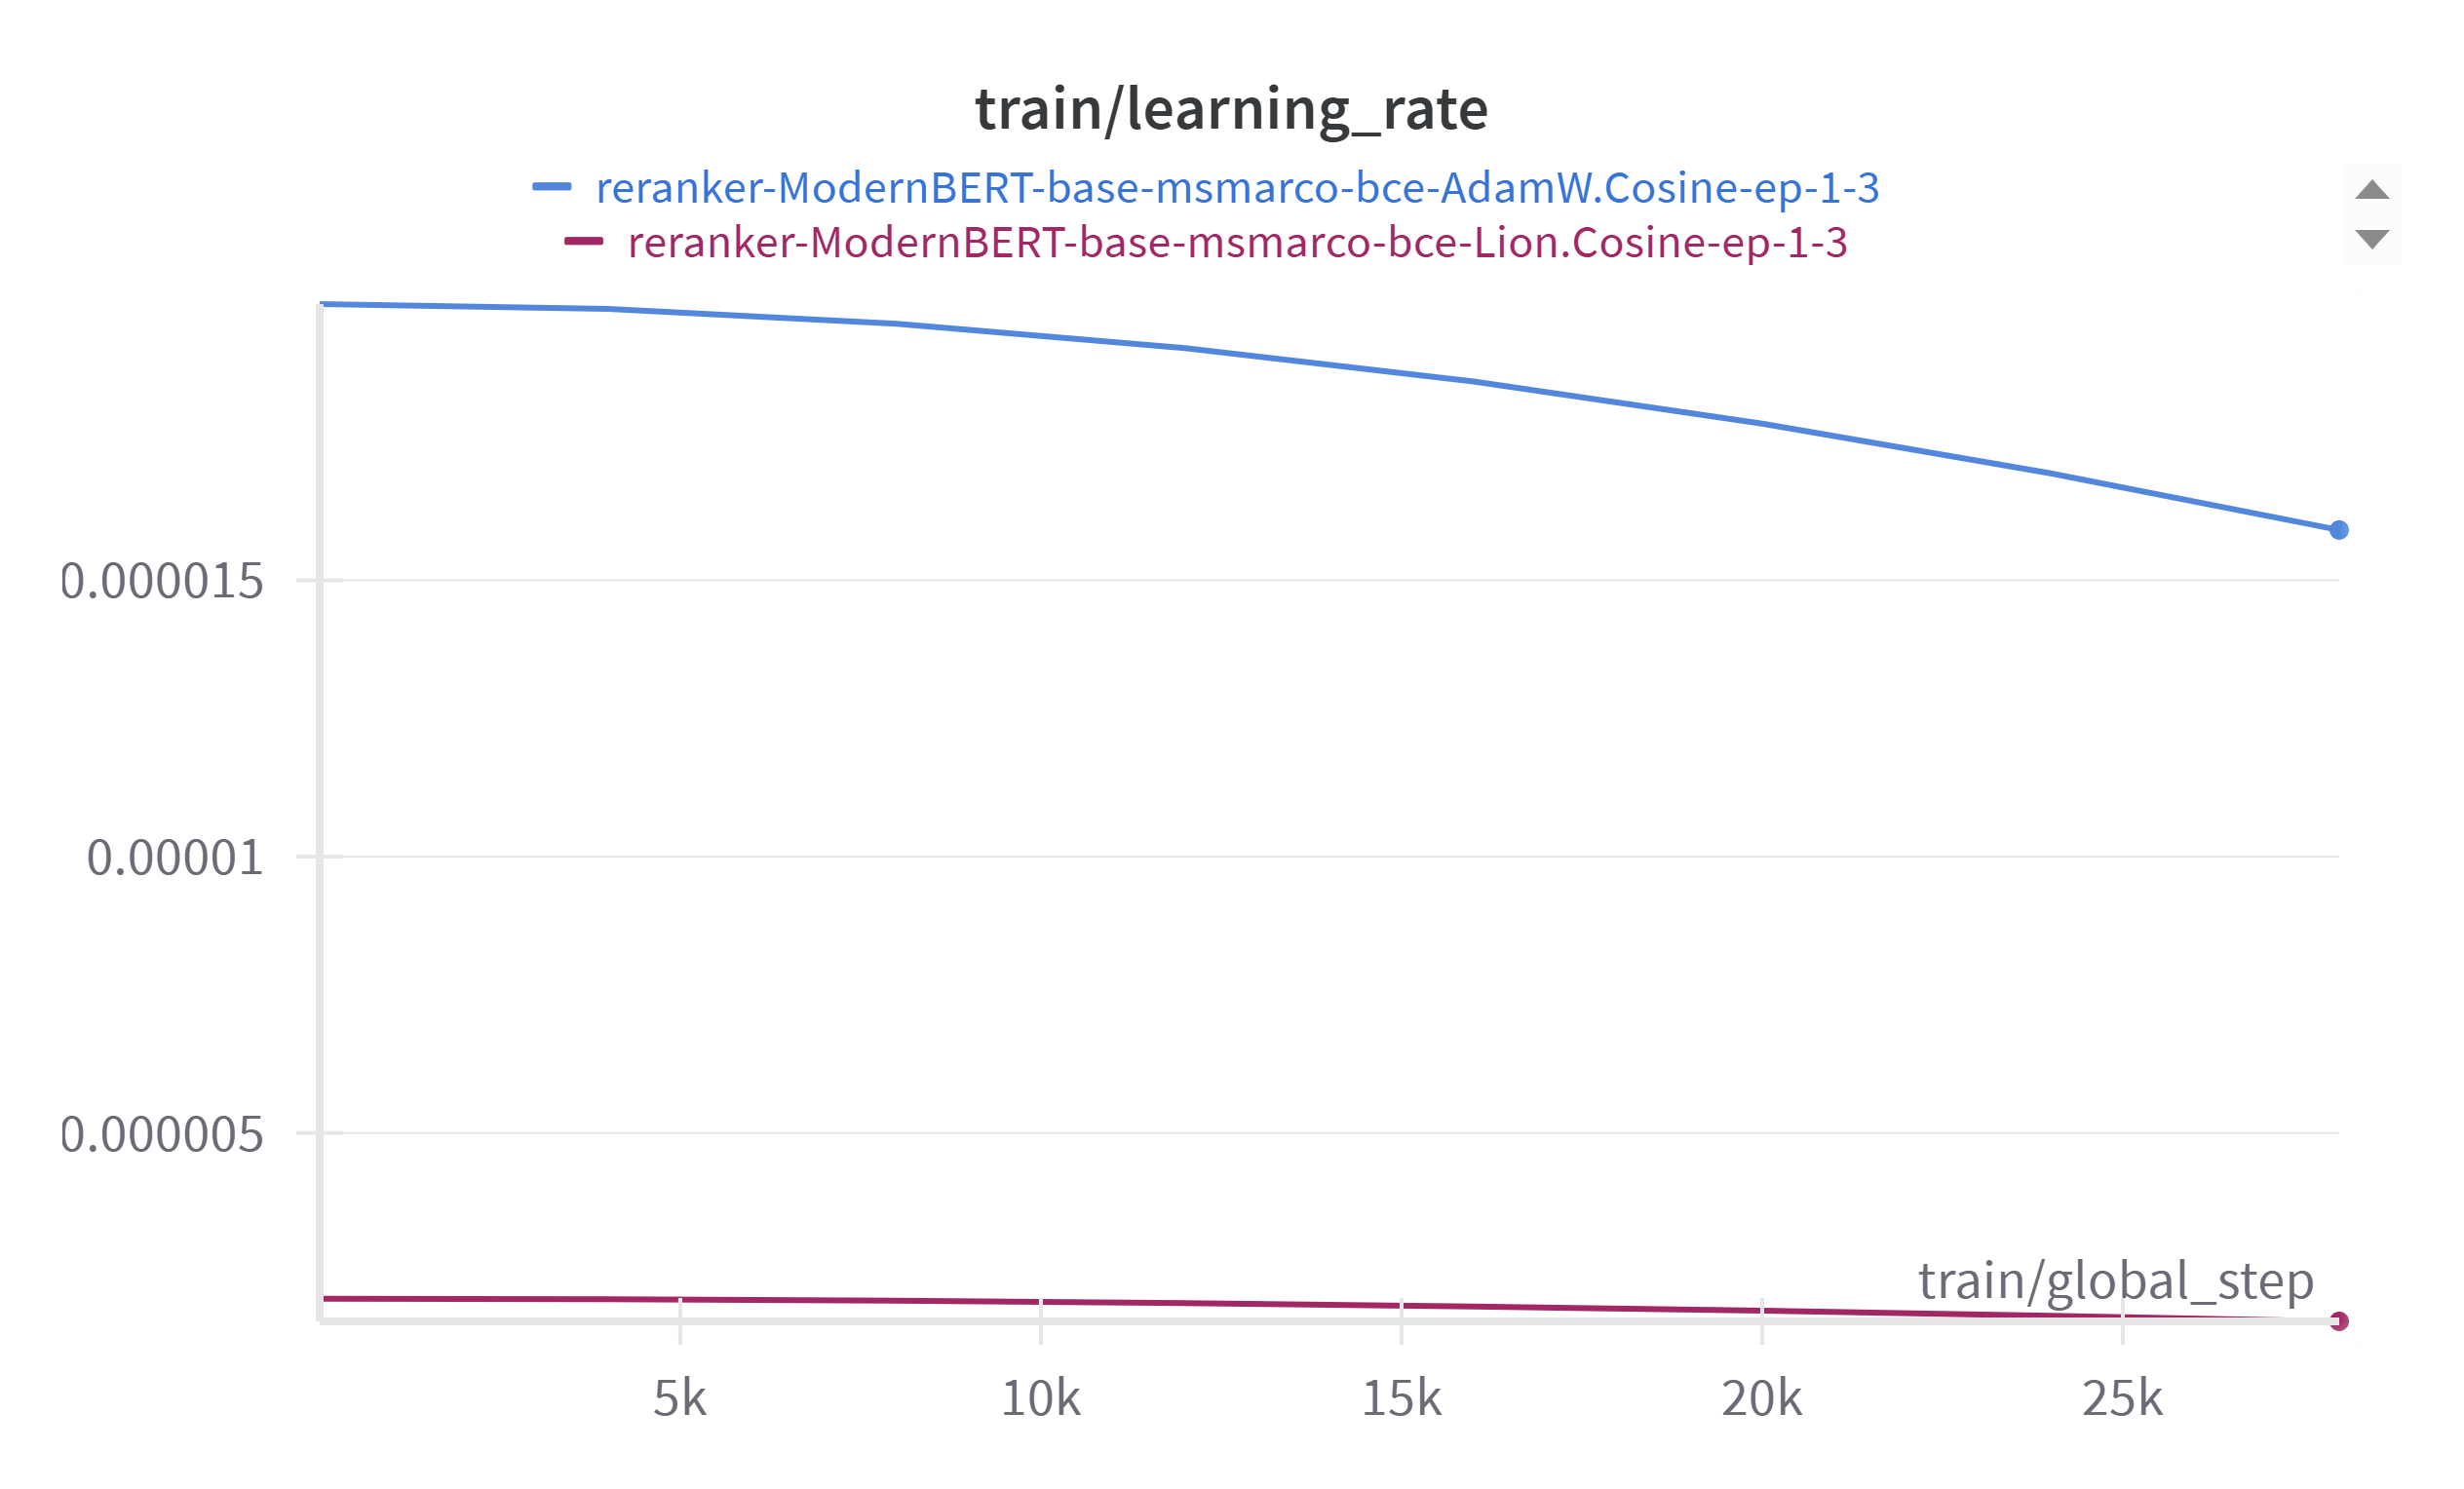
\includegraphics[width=\linewidth]{figures/modernBERT-Lion-adamW-lrate.png}
    \caption{Learning Rate}
    \label{fig:modernbert_lr}
\end{subfigure}
\hfill
\begin{subfigure}[b]{0.45\textwidth}
    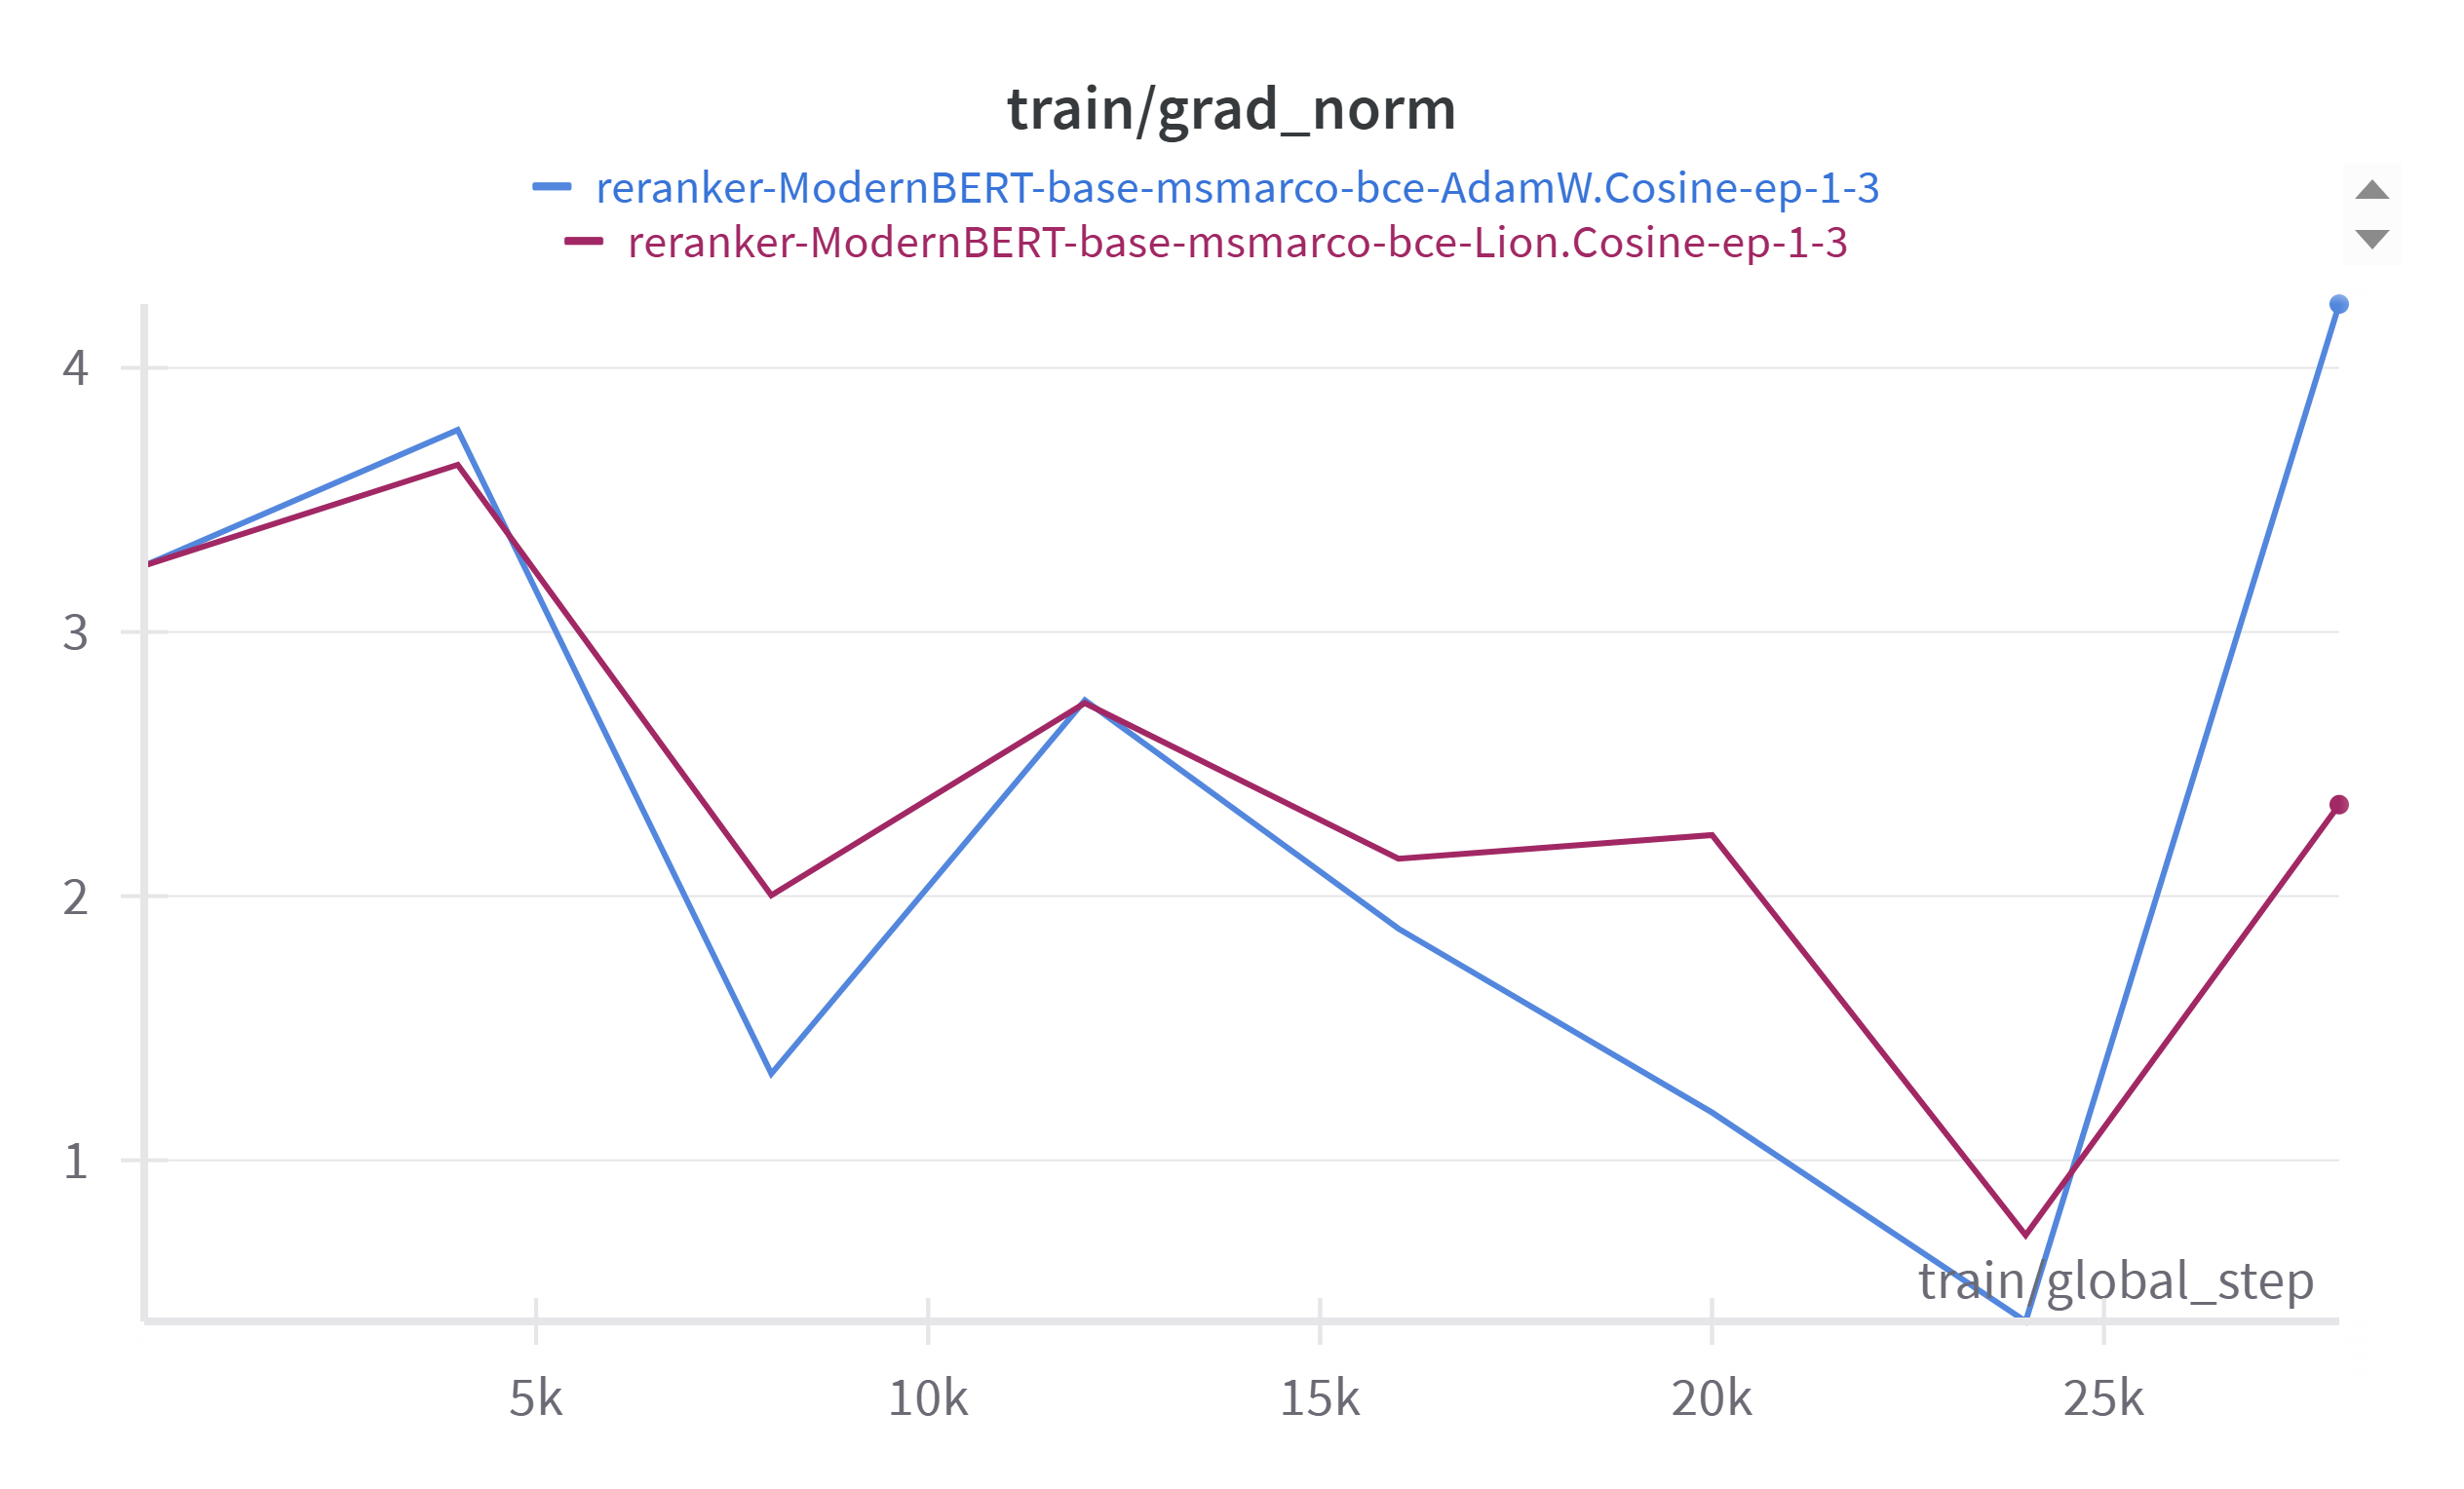
\includegraphics[width=\linewidth]{figures/modernBERT-Lion-adamW_grad.png}
    \caption{Gradient Norm}
    \label{fig:modernbert_grad}
\end{subfigure}

\caption{Training Dynamics for ModernBERT-base with Lion and AdamW optimizers. Each plot shows a different training metric over training steps.}
\label{fig:modernbert_training_plots}
\end{figure*}



\subsection{Comparison with State-of-the-Art}
Table \ref{tab:sota_comparison} situates our best result (ModernBERT + Lion, Epoch 2) relative to other published results on TREC DL 2019 passage ranking.

% \begin{table}[htbp]
% \centering
% \caption{Comparison with Other Systems on TREC DL 2019 (NDCG@10)}
% \label{tab:sota_comparison}
% \begin{tabular}{l c c}
% \toprule
% \textbf{Model/System} & \textbf{NDCG@10} & \textbf{Reference} \\
% \midrule
% \midrule
% \textit{Sparse Retrieval (single stage} & & \\
% \midrule
% BM25 & 0.506 & \cite{lin2020distill} \\
% DeepCT & 0.551 & \cite{gao2021complementing}\\
% doc2query-T5 & 0.642 & \cite{Lin2021PretrainedTF} \\
% \midrule
% \textit{Dense Retrieval Models} & & \\
% \midrule
% ANCE & 0.648 & \cite{xiong2020approximate} \\
% Rand Neg & 0.605 & \cite{xiong2020approximate} \\
% NCE Neg & 0.602 & \cite{xiong2020approximate} \\
% BM25 Neg & 0.664 & \cite{xiong2020approximate} \\
% DPR (BM25 + Rand Neg) & 0.653 & \cite{xiong2020approximate} \\
% BM25 $\rightarrow$ Rand & 0.609 & \cite{xiong2020approximate} \\
% BM25 $\rightarrow$ NCE Neg & 0.608 & \cite{xiong2020approximate} \\
% BM25 $\rightarrow$ BM25 + Rand & 0.648 & \cite{xiong2020approximate} \\
% \midrule
% \textit{Hybrid dense + sparse (single stage} & & \\
% \midrule
% Bi-encoder (PoolAvg) + BM25 & 0.701 & \cite{lin2020distill} \\
% Bi-encoder (TCT-ColBERT) + BM25 & 0.714 & \cite{lin2020distill} \\
% Bi-encoder (PoolAvg) + doc2query-T5 & 0.719 & \cite{lin2020distill} \\
% \midrule
% \textit{Cross-Encoder/Reranking Models} & & \\
% \midrule
% BERT-base Cross-Encoder & 0.634 & \cite{Lin2021PretrainedTF} \\
% BERT-large Cross-Encoder & 0.654 & \cite{Lin2021PretrainedTF} \\
% pt-bert-base-uncased-msmarco & 0.709 & \cite{koursaros2019NBoost} \\
% cross-encoder/ms-marco-electra-base & 0.0.7199 & \cite{reimers2019sentence} \\
% cross-encoder/ms-marco-TinyBERT-L-2-v2 & 0.6984 & \cite{reimers2019sentence} \\
% \midrule
% \textbf{Our Best (ModernBERT+Lion E2)} & \textbf{0.7225} & This work \\
% \textbf{Our GTE+AdamW E1/E2} & \textbf{0.7224} / 0.7203 & This work \\
% \textbf{Our MiniLM+AdamW E3} & 0.7127 & This work \\
% \bottomrule
% \end{tabular}
% \vspace{1em}\\
% \footnotesize{Various references cited in text. Some metrics may vary slightly based on specific evaluation setup or version.}
% \end{table}

% Our best model, ModernBERT+Lion (NDCG@10 = 0.7225), significantly outperforms the BM25 baseline and standard BERT-base/large cross-encoders reported in \cite{Lin2021PretrainedTF}. It achieves performance comparable to or exceeding strong dense retrieval models like TAS-B and reported base-size bi-encoders \cite{zhan2024scaling}, and also exceeds some reported BERT-base cross-encoder results \cite{koursaros2019NBoost}. Our GTE+AdamW model achieves nearly identical peak performance. While not reaching the level of very large models like MonoT5-3B or specialized architectures like ColBERT, our results demonstrate strong performance using base-sized models with appropriate optimizer choices and training strategies.

\begin{table}[htbp]
\centering
\caption{Comparison with Other Systems on TREC DL 2019 (NDCG@10)}
\label{tab:sota_comparison}
\begin{tabular}{l c c}
\toprule
\textbf{Model/System} & \textbf{NDCG@10} & \textbf{Reference} \\
\midrule
\midrule
\textbf{Sparse Retrieval (single stage)} & & \\
\midrule
BM25 & 0.506 & \cite{lin2020distill} \\
DeepCT & 0.551 & \cite{gao2021complementing} \\
doc2query-T5 & 0.642 & \cite{Lin2021PretrainedTF} \\
\midrule
\textbf{Dense Retrieval Models} & & \\
\midrule
ANCE & 0.648 & \cite{xiong2020approximate} \\
Rand Neg & 0.605 & \cite{xiong2020approximate} \\
NCE Neg & 0.602 & \cite{xiong2020approximate} \\
BM25 Neg & 0.664 & \cite{xiong2020approximate} \\
DPR (BM25 + Rand Neg) & 0.653 & \cite{xiong2020approximate} \\
BM25 $\rightarrow$ Rand & 0.609 & \cite{xiong2020approximate} \\
BM25 $\rightarrow$ NCE Neg & 0.608 & \cite{xiong2020approximate} \\
BM25 $\rightarrow$ BM25 + Rand & 0.648 & \cite{xiong2020approximate} \\
\midrule
\textbf{Hybrid dense + sparse (single stage)} & & \\
\midrule
Bi-encoder (PoolAvg) + BM25 & 0.701 & \cite{lin2020distill} \\
Bi-encoder (TCT-ColBERT) + BM25 & 0.714 & \cite{lin2020distill} \\
Bi-encoder (PoolAvg) + doc2query-T5 & 0.719 & \cite{lin2020distill} \\
\midrule
\textbf{Cross-Encoder/Reranking Models} & & \\
\midrule
BERT-base Cross-Encoder & 0.634 & \cite{Lin2021PretrainedTF} \\
BERT-large Cross-Encoder & 0.654 & \cite{Lin2021PretrainedTF} \\
pt-bert-base-uncased-msmarco & 0.709 & \cite{koursaros2019NBoost} \\
cross-encoder/ms-marco-electra-base & 0.719 & \cite{reimers2019sentence} \\
cross-encoder/ms-marco-TinyBERT-L-2-v2 & 0.698 & \cite{reimers2019sentence} \\
\midrule
\textbf{Our Best (ModernBERT+Lion E2)} & \textbf{0.7225} & This work \\
\textbf{Our GTE+AdamW E1/E2} & \textbf{0.7224} / 0.7203 & This work \\
\textbf{Our MiniLM+AdamW E3} & 0.7127 & This work \\
\bottomrule
\end{tabular}
\vspace{1em}\\
\footnotesize{NDCG@10 scores are reported as evaluated on the TREC DL 2019 dataset using standard settings from cited references. Minor variations may occur due to differences in implementation, random seeds, or reranking candidate sets.}
\end{table}

Our best model, ModernBERT+Lion (NDCG@10 = 0.7225), achieves the highest performance among the models listed in Table \ref{tab:sota_comparison}, surpassing strong baselines such as BM25 (0.506), dense retrieval models like ANCE (0.648) and BM25 Neg (0.664), hybrid models such as Bi-encoder (PoolAvg) + doc2query-T5 (0.719), and cross-encoder models including cross-encoder/ms-marco-electra-base (0.7199). Our GTE+AdamW model achieves nearly identical performance (0.7224), while our MiniLM+AdamW variant scores 0.7127, remaining competitive. These results highlight the effectiveness of our optimizer choices and training strategies for base-sized models.

\section{Conclusion}
\label{sec:conclusion}
In this paper, we presented a comparative study of the Lion and AdamW optimizers for fine-tuning three different transformer models (`microsoft/MiniLM-L12-H384-uncased`, `Alibaba-NLP/gte-multilingual-base`, `answerdotai/ModernBERT-base`) as cross-encoders for passage reranking. Training was performed on MS MARCO, and evaluation used TREC 2019 Deep Learning Track and MS MARCO dev benchmarks. Our findings indicate:
\begin{itemize}
    \item The choice of optimizer significantly interacts with the base model and training hyperparameters (LR, scheduler).
    \item For ModernBERT, using a low learning rate (2e-6) and Cosine Annealing scheduler, Lion substantially outperformed AdamW, achieving the best overall TREC DL 2019 results (NDCG@10 = 0.7225, MAP = 0.5121 at Epochs 1-2).
    \item For GTE, AdamW (with LR 2e-5, no scheduler) was more effective than Lion, achieving strong results (NDCG@10 = 0.7224) comparable to ModernBERT+Lion.
    \item For MiniLM, AdamW yielded slightly better TREC performance over 3 epochs, while Lion achieved the best MS MARCO dev MRR@10 (tied with ModernBERT+Lion).
    \item Models with longer context capabilities (GTE, ModernBERT) generally outperformed MiniLM on the TREC DL task.
    \item Performance varied across epochs, emphasizing the need for checkpoint selection based on validation performance.
\end{itemize}
Our results show that Lion can be a highly effective optimizer for cross-encoder training, particularly for newer architectures like ModernBERT when paired with appropriate learning rate strategies. However, AdamW remains a strong baseline, especially for models like GTE in this setup. The Modal platform proved effective for managing the required GPU resources and experimental setup.

Future work could involve a more thorough hyperparameter search for both optimizers across all models, particularly exploring different learning rates and schedules for Lion with MiniLM and GTE. Investigating the impact of the 8K context length more directly (e.g., on datasets with longer documents) and analyzing memory usage differences between optimizers would also be valuable.

\section*{Acknowledgment}
The authors acknowledge Modal Labs (\url{https://modal.com/}) for providing the cloud computing platform and GPU(s) resources (NVIDIA A100-80GB) used for conducting the experiments presented in this paper.

% --- Bibliography ---
\bibliographystyle{IEEEtran}
\bibliography{IEEEabrv,references} 

\appendix

\section{Detailed Evaluation Metrics}
\label{app:metrics}

This appendix presents comprehensive evaluation metrics for all model configurations tested in our experiments. While the main paper focuses on key performance indicators, these detailed tables provide additional insights into model behavior across various retrieval effectiveness measures.

\subsection{Primary Ranking Metrics}
Table~\ref{tab:primary_metrics} presents the main effectiveness metrics including MAP, NDCG@10, MRR@10, and Precision@10 for all tested configurations.

\subsection{Precision and Recall Analysis}
Tables~\ref{tab:precision_metrics} and~\ref{tab:recall_metrics} provide detailed precision and recall values at different cutoff thresholds, revealing the models' behavior at various result list depths.

\subsection{NDCG and MAP Metrics}
Tables~\ref{tab:ndcg_metrics} and~\ref{tab:map_metrics} provide a more granular view of ranking quality through normalized discounted cumulative gain and mean average precision at multiple cutoff points.

\subsection{Advanced Retrieval Metrics}
Table~\ref{tab:interpolated_precision} presents R-Precision and interpolated precision metrics that provide insights into precision at different recall levels.

\subsection{User-Focused Metrics}
Table~\ref{tab:success_metrics} presents metrics that focus on user satisfaction, including success rates and rank-biased precision.

\subsection{Metric Definitions}
\label{app:metric_defs}
Table~\ref{tab:metric_definitions} provides formal definitions of all evaluation metrics used in our experimental analysis.

\begin{table*}[t]
\centering
\caption{Primary ranking metrics comparing cross-encoder models across training epochs.}
\label{tab:primary_metrics}
\small
\begin{tabular}{llcccccccc}
\toprule
\textbf{Model} & \textbf{Optimizer} & \textbf{Epoch} & \textbf{MAP} & \textbf{NDCG@10} & \textbf{MRR@10} & \textbf{P@10} & \textbf{Recip\_Rank} & \textbf{R-Prec} & \textbf{bpref} \\
\midrule
\multirow{6}{*}{GTE} & \multirow{3}{*}{AdamW} 
 & 1 & 0.5005 & 0.7224 & 0.5940 & 0.8116 & 0.9814 & 0.4964 & 0.6068 \\
 & & 2 & 0.4999 & 0.7203 & 0.5942 & 0.8256 & 0.9523 & 0.5018 & 0.6074 \\
 & & 3 & 0.4899 & 0.6902 & 0.5972 & 0.8093 & 0.9279 & 0.5017 & 0.6075 \\
\cmidrule{2-10}
 & \multirow{3}{*}{Lion} 
 & 1 & 0.4794 & 0.6970 & 0.5854 & 0.7884 & 0.9612 & 0.4814 & 0.6079 \\
 & & 2 & 0.4577 & 0.6792 & 0.5957 & 0.7721 & 0.9477 & 0.4642 & 0.6013 \\
 & & 3 & 0.4521 & 0.6571 & 0.5931 & 0.7488 & 0.9399 & 0.4662 & 0.5972 \\
\midrule
\multirow{6}{*}{MiniLM} & \multirow{3}{*}{AdamW} 
 & 1 & 0.4814 & 0.7008 & 0.5828 & 0.8000 & 0.9465 & 0.4884 & 0.6016 \\
 & & 2 & 0.4891 & 0.7094 & 0.5818 & 0.8116 & 0.9814 & 0.4916 & 0.6030 \\
 & & 3 & 0.4908 & 0.7127 & 0.5826 & 0.8116 & 0.9806 & 0.4943 & 0.6048 \\
\cmidrule{2-10}
 & \multirow{3}{*}{Lion} 
 & 1 & 0.4858 & 0.7031 & 0.5890 & 0.8140 & 0.9457 & 0.4952 & 0.6010 \\
 & & 2 & 0.4755 & 0.6916 & 0.5942 & 0.8070 & 0.9496 & 0.4803 & 0.5992 \\
 & & 3 & 0.4706 & 0.6808 & \textbf{0.5988} & 0.8070 & 0.9419 & 0.4809 & 0.5994 \\
\midrule
\multirow{6}{*}{ModernBERT} & \multirow{3}{*}{AdamW} 
 & 1 & 0.5066 & 0.7105 & 0.5866 & 0.8163 & 0.9574 & 0.5161 & 0.6139 \\
 & & 2 & 0.4893 & 0.6839 & 0.5886 & 0.7814 & 0.9341 & 0.4946 & 0.6152 \\
 & & 3 & 0.4971 & 0.6959 & 0.5916 & 0.7860 & 0.9523 & 0.5116 & 0.6128 \\
\cmidrule{2-10}
 & \multirow{3}{*}{Lion} 
 & 1 & 0.5121 & 0.7142 & 0.5834 & 0.8163 & 0.9593 & 0.5148 & 0.6140 \\
 & & 2 & \textbf{0.5115} & \textbf{0.7225} & 0.5908 & \textbf{0.8209} & \textbf{0.9767} & \textbf{0.5183} & \textbf{0.6156} \\
 & & 3 & 0.5020 & 0.7051 & 0.5989 & 0.8256 & 0.9322 & 0.5102 & 0.6151 \\
\bottomrule
\end{tabular}
\end{table*}



\begin{table*}[t]
\centering
\caption{Precision metrics at different cutoff levels.}
\label{tab:precision_metrics}
\small
\begin{tabular}{llccccccc}
\toprule
\textbf{Model} & \textbf{Config} & \textbf{P@5} & \textbf{P@10} & \textbf{P@15} & \textbf{P@20} & \textbf{P@30} & \textbf{P@100} & \textbf{P@200} \\
\midrule
\multirow{6}{*}{GTE} & AdamW-1 & 0.8930 & 0.8116 & 0.7783 & 0.7372 & 0.6419 & 0.3965 & 0.2664 \\
 & AdamW-2 & 0.8698 & 0.8256 & 0.7752 & 0.7326 & 0.6395 & 0.3963 & 0.2641 \\
 & AdamW-3 & 0.8558 & 0.8093 & 0.7550 & 0.7128 & 0.6349 & 0.3942 & 0.2634 \\
 & Lion-1 & 0.8558 & 0.7884 & 0.7364 & 0.7070 & 0.6318 & 0.3893 & 0.2591 \\
 & Lion-2 & 0.8326 & 0.7721 & 0.7302 & 0.6802 & 0.6054 & 0.3740 & 0.2528 \\
 & Lion-3 & 0.8140 & 0.7488 & 0.7147 & 0.6907 & 0.6140 & 0.3740 & 0.2543 \\
\midrule
\multirow{6}{*}{MiniLM} & AdamW-1 & 0.8698 & 0.8000 & 0.7628 & 0.7151 & 0.6450 & 0.3870 & 0.2564 \\
 & AdamW-2 & 0.8698 & 0.8116 & 0.7674 & 0.7186 & 0.6488 & 0.3895 & 0.2580 \\
 & AdamW-3 & 0.8558 & 0.8116 & 0.7705 & 0.7256 & 0.6442 & 0.3891 & 0.2580 \\
 & Lion-1 & 0.8651 & 0.8140 & 0.7783 & 0.7233 & 0.6434 & 0.3847 & 0.2583 \\
 & Lion-2 & 0.8744 & 0.8070 & 0.7643 & 0.7081 & 0.6264 & 0.3821 & 0.2530 \\
 & Lion-3 & 0.8465 & 0.8070 & 0.7442 & 0.6930 & 0.6194 & 0.3809 & 0.2547 \\
\midrule
\multirow{6}{*}{ModernBERT} & AdamW-1 & 0.8651 & 0.8163 & 0.7767 & 0.7349 & 0.6612 & 0.3993 & 0.2679 \\
 & AdamW-2 & 0.8605 & 0.7814 & 0.7333 & 0.6953 & 0.6333 & 0.3912 & 0.2658 \\
 & AdamW-3 & 0.8465 & 0.7860 & 0.7411 & 0.6988 & 0.6450 & 0.3958 & 0.2655 \\
 & Lion-1 & 0.8791 & 0.8163 & 0.7783 & 0.7314 & 0.6574 & 0.4033 & 0.2691 \\
 & Lion-2 & 0.8698 & \textbf{0.8209} & 0.7674 & 0.7279 & 0.6574 & \textbf{0.4016} & 0.2678 \\
 & Lion-3 & 0.8651 & 0.8256 & 0.7504 & 0.7093 & 0.6488 & 0.3967 & 0.2651 \\
\bottomrule
\end{tabular}
\end{table*}

\begin{table*}[t]
\centering
\caption{Recall metrics at different cutoff levels.}
\label{tab:recall_metrics}
\small
\begin{tabular}{llcccccccc}
\toprule
\textbf{Model} & \textbf{Config} & \textbf{Recall@5} & \textbf{Recall@10} & \textbf{Recall@15} & \textbf{Recall@20} & \textbf{Recall@30} & \textbf{Recall@100} & \textbf{Recall@200} & \textbf{Recall@500} \\
\midrule
\multirow{6}{*}{GTE} & AdamW-1 & 0.1051 & 0.1689 & 0.2286 & 0.2815 & 0.3376 & 0.5501 & 0.6573 & 0.7161 \\
 & AdamW-2 & 0.1041 & 0.1760 & 0.2295 & 0.2753 & 0.3366 & 0.5538 & 0.6511 & 0.7130 \\
 & AdamW-3 & 0.1051 & 0.1715 & 0.2256 & 0.2692 & 0.3376 & 0.5489 & 0.6501 & 0.7102 \\
 & Lion-1 & 0.1002 & 0.1614 & 0.2158 & 0.2684 & 0.3369 & 0.5401 & 0.6384 & 0.7101 \\
 & Lion-2 & 0.0973 & 0.1610 & 0.2151 & 0.2545 & 0.3153 & 0.5211 & 0.6273 & 0.7105 \\
 & Lion-3 & 0.0929 & 0.1542 & 0.2070 & 0.2574 & 0.3221 & 0.5181 & 0.6227 & 0.7124 \\
\midrule
\multirow{6}{*}{MiniLM} & AdamW-1 & 0.1027 & 0.1652 & 0.2225 & 0.2645 & 0.3362 & 0.5426 & 0.6396 & 0.7187 \\
 & AdamW-2 & 0.1013 & 0.1668 & 0.2239 & 0.2676 & 0.3401 & 0.5446 & 0.6417 & 0.7223 \\
 & AdamW-3 & 0.1007 & 0.1702 & 0.2257 & 0.2719 & 0.3386 & 0.5427 & 0.6396 & 0.7189 \\
 & Lion-1 & 0.1022 & 0.1688 & 0.2257 & 0.2704 & 0.3400 & 0.5338 & 0.6413 & 0.7154 \\
 & Lion-2 & 0.1025 & 0.1641 & 0.2200 & 0.2613 & 0.3289 & 0.5338 & 0.6268 & 0.7145 \\
 & Lion-3 & 0.1001 & 0.1676 & 0.2156 & 0.2542 & 0.3253 & 0.5249 & 0.6341 & 0.7143 \\
\midrule
\multirow{6}{*}{ModernBERT} & AdamW-1 & 0.0995 & 0.1678 & 0.2245 & 0.2731 & 0.3475 & 0.5520 & 0.6539 & 0.7224 \\
 & AdamW-2 & 0.0979 & 0.1634 & 0.2148 & 0.2603 & 0.3321 & 0.5443 & 0.6520 & 0.7198 \\
 & AdamW-3 & 0.1019 & 0.1623 & 0.2184 & 0.2627 & 0.3380 & 0.5476 & 0.6461 & 0.7198 \\
 & Lion-1 & 0.1052 & 0.1689 & 0.2276 & 0.2733 & 0.3431 & 0.5542 & 0.6553 & 0.7233 \\
 & Lion-2 & 0.1048 & \textbf{0.1732} & 0.2245 & 0.2699 & 0.3469 & \textbf{0.5608} & \textbf{0.6553} & \textbf{0.7233} \\
 & Lion-3 & 0.1037 & 0.1722 & 0.2185 & 0.2640 & 0.3425 & 0.5570 & 0.6525 & 0.7194 \\
\bottomrule
\end{tabular}
\end{table*}



\begin{table*}[t]
\centering
\caption{NDCG metrics at different cutoff levels.}
\label{tab:ndcg_metrics}
\small
\begin{tabular}{llccccccc}
\toprule
\textbf{Model} & \textbf{Config} & \textbf{NDCG} & \textbf{NDCG@5} & \textbf{NDCG@10} & \textbf{NDCG@20} & \textbf{NDCG@30} & \textbf{NDCG@100} & \textbf{NDCG@500} \\
\midrule
\multirow{6}{*}{GTE} & AdamW-1 & 0.6987 & 0.7567 & 0.7224 & 0.7071 & 0.6802 & 0.6591 & 0.6897 \\
 & AdamW-2 & 0.6949 & 0.7343 & 0.7203 & 0.6967 & 0.6687 & 0.6550 & 0.6845 \\
 & AdamW-3 & 0.6848 & 0.7080 & 0.6902 & 0.6703 & 0.6558 & 0.6426 & 0.6733 \\
 & Lion-1 & 0.6865 & 0.7229 & 0.6970 & 0.6786 & 0.6638 & 0.6433 & 0.6750 \\
 & Lion-2 & 0.6772 & 0.7008 & 0.6792 & 0.6580 & 0.6405 & 0.6248 & 0.6661 \\
 & Lion-3 & 0.6674 & 0.6801 & 0.6571 & 0.6450 & 0.6310 & 0.6124 & 0.6573 \\
\midrule
\multirow{6}{*}{MiniLM} & AdamW-1 & 0.6857 & 0.7207 & 0.7008 & 0.6833 & 0.6698 & 0.6402 & 0.6778 \\
 & AdamW-2 & 0.6910 & 0.7345 & 0.7094 & 0.6908 & 0.6779 & 0.6471 & 0.6843 \\
 & AdamW-3 & 0.6910 & 0.7244 & 0.7127 & 0.6949 & 0.6749 & 0.6474 & 0.6834 \\
 & Lion-1 & 0.6841 & 0.7163 & 0.7031 & 0.6829 & 0.6667 & 0.6369 & 0.6752 \\
 & Lion-2 & 0.6790 & 0.7099 & 0.6916 & 0.6706 & 0.6541 & 0.6295 & 0.6692 \\
 & Lion-3 & 0.6770 & 0.6837 & 0.6808 & 0.6584 & 0.6479 & 0.6268 & 0.6667 \\
\midrule
\multirow{6}{*}{ModernBERT} & AdamW-1 & 0.6937 & 0.7171 & 0.7105 & 0.6936 & 0.6831 & 0.6555 & 0.6877 \\
 & AdamW-2 & 0.6869 & 0.7112 & 0.6839 & 0.6701 & 0.6589 & 0.6431 & 0.6795 \\
 & AdamW-3 & 0.6910 & 0.7156 & 0.6959 & 0.6729 & 0.6699 & 0.6497 & 0.6832 \\
 & Lion-1 & 0.6984 & 0.7285 & 0.7142 & 0.6991 & 0.6825 & 0.6610 & 0.6925 \\
 & Lion-2 & \textbf{0.7018} & \textbf{0.7381} & \textbf{0.7225} & \textbf{0.6978} & \textbf{0.6852} & \textbf{0.6638} & \textbf{0.6955} \\
 & Lion-3 & 0.6930 & 0.7165 & 0.7051 & 0.6797 & 0.6722 & 0.6542 & 0.6857 \\
\bottomrule
\end{tabular}
\end{table*}

\begin{table*}[t]
\centering
\caption{MAP metrics at different cutoff levels and related metrics.}
\label{tab:map_metrics}
\small
\begin{tabular}{llccccccc}
\toprule
\textbf{Model} & \textbf{Config} & \textbf{MAP} & \textbf{MAP@10} & \textbf{MAP@20} & \textbf{MAP@30} & \textbf{MAP@100} & \textbf{infAP} & \textbf{gm\_map} \\
\midrule
\multirow{6}{*}{GTE} & AdamW-1 & 0.5005 & 0.1601 & 0.2499 & 0.2915 & 0.4226 & 0.5005 & 0.4143 \\
 & AdamW-2 & 0.4999 & 0.1632 & 0.2463 & 0.2904 & 0.4247 & 0.4999 & 0.4109 \\
 & AdamW-3 & 0.4899 & 0.1555 & 0.2350 & 0.2827 & 0.4136 & 0.4899 & 0.3995 \\
 & Lion-1 & 0.4794 & 0.1468 & 0.2274 & 0.2771 & 0.4039 & 0.4794 & 0.3878 \\
 & Lion-2 & 0.4577 & 0.1464 & 0.2201 & 0.2631 & 0.3810 & 0.4577 & 0.3623 \\
 & Lion-3 & 0.4521 & 0.1378 & 0.2145 & 0.2589 & 0.3747 & 0.4521 & 0.3525 \\
\midrule
\multirow{6}{*}{MiniLM} & AdamW-1 & 0.4814 & 0.1479 & 0.2272 & 0.2809 & 0.4062 & 0.4814 & 0.3920 \\
 & AdamW-2 & 0.4891 & 0.1531 & 0.2329 & 0.2882 & 0.4148 & 0.4891 & 0.3975 \\
 & AdamW-3 & 0.4908 & 0.1553 & 0.2383 & 0.2895 & 0.4159 & 0.4908 & 0.3972 \\
 & Lion-1 & 0.4858 & 0.1534 & 0.2344 & 0.2845 & 0.4087 & 0.4858 & 0.3919 \\
 & Lion-2 & 0.4755 & 0.1492 & 0.2254 & 0.2735 & 0.4006 & 0.4755 & 0.3823 \\
 & Lion-3 & 0.4706 & 0.1507 & 0.2207 & 0.2690 & 0.3940 & 0.4706 & 0.3736 \\
\midrule
\multirow{6}{*}{ModernBERT} & AdamW-1 & 0.5066 & 0.1535 & 0.2389 & 0.2942 & 0.4274 & 0.5066 & 0.4045 \\
 & AdamW-2 & 0.4893 & 0.1493 & 0.2280 & 0.2803 & 0.4097 & 0.4893 & 0.3875 \\
 & AdamW-3 & 0.4971 & 0.1504 & 0.2304 & 0.2848 & 0.4192 & 0.4971 & 0.3988 \\
 & Lion-1 & 0.5121 & 0.1577 & 0.2448 & 0.2979 & 0.4347 & 0.5121 & 0.4162 \\
 & Lion-2 & \textbf{0.5115} & \textbf{0.1616} & \textbf{0.2417} & \textbf{0.2973} & \textbf{0.4333} & \textbf{0.5115} & \textbf{0.4157} \\
 & Lion-3 & 0.5020 & 0.1583 & 0.2333 & 0.2892 & 0.4239 & 0.5020 & 0.4071 \\
\bottomrule
\end{tabular}
\end{table*}



\begin{table*}[t]
\centering
\caption{R-Precision and interpolated precision metrics.}
\label{tab:interpolated_precision}
\small
\resizebox{\textwidth}{!}{%
\begin{tabular}{llccccccccc}
\toprule
\textbf{Model} & \textbf{Config} & \textbf{R-Prec} & \textbf{R-Prec@0.8} & \textbf{R-Prec@1.0} & \textbf{iprec@0.0} & \textbf{iprec@0.1} & \textbf{iprec@0.3} & \textbf{iprec@0.5} & \textbf{iprec@0.7} & \textbf{iprec@0.9} \\
\midrule
\multirow{6}{*}{GTE} & AdamW-1 & 0.4964 & 0.5617 & 0.4964 & 0.9841 & 0.8741 & 0.7176 & 0.5037 & 0.3295 & 0.1439 \\
 & AdamW-2 & 0.5018 & 0.5644 & 0.5018 & 0.9730 & 0.8796 & 0.7093 & 0.5027 & 0.3339 & 0.1399 \\
 & AdamW-3 & 0.5017 & 0.5616 & 0.5017 & 0.9611 & 0.8614 & 0.6942 & 0.4980 & 0.3404 & 0.1395 \\
 & Lion-1 & 0.4814 & 0.5419 & 0.4814 & 0.9667 & 0.8426 & 0.6601 & 0.4907 & 0.3576 & 0.1233 \\
 & Lion-2 & 0.4642 & 0.5238 & 0.4642 & 0.9682 & 0.8377 & 0.6283 & 0.4549 & 0.3144 & 0.1182 \\
 & Lion-3 & 0.4662 & 0.5236 & 0.4662 & 0.9519 & 0.8008 & 0.6289 & 0.4653 & 0.3158 & 0.1218 \\
\midrule
\multirow{6}{*}{MiniLM} & AdamW-1 & 0.4884 & 0.5502 & 0.4884 & 0.9637 & 0.8546 & 0.6592 & 0.4804 & 0.3474 & 0.1258 \\
 & AdamW-2 & 0.4916 & 0.5523 & 0.4916 & 0.9821 & 0.8584 & 0.6614 & 0.4856 & 0.3537 & 0.1251 \\
 & AdamW-3 & 0.4943 & 0.5611 & 0.4943 & 0.9817 & 0.8641 & 0.6724 & 0.4877 & 0.3469 & 0.1262 \\
 & Lion-1 & 0.4952 & 0.5495 & 0.4952 & 0.9727 & 0.8613 & 0.6698 & 0.4836 & 0.3387 & 0.1326 \\
 & Lion-2 & 0.4803 & 0.5335 & 0.4803 & 0.9728 & 0.8450 & 0.6441 & 0.4545 & 0.3422 & 0.1261 \\
 & Lion-3 & 0.4809 & 0.5240 & 0.4809 & 0.9625 & 0.8511 & 0.6443 & 0.4543 & 0.3370 & 0.1278 \\
\midrule
\multirow{6}{*}{ModernBERT} & AdamW-1 & 0.5161 & 0.5804 & 0.5161 & 0.9688 & 0.8676 & 0.6739 & 0.5126 & 0.3858 & 0.1644 \\
 & AdamW-2 & 0.4946 & 0.5492 & 0.4946 & 0.9583 & 0.8429 & 0.6547 & 0.4956 & 0.3741 & 0.1464 \\
 & AdamW-3 & 0.5116 & 0.5638 & 0.5116 & 0.9614 & 0.8460 & 0.6781 & 0.5001 & 0.3774 & 0.1489 \\
 & Lion-1 & 0.5148 & 0.5848 & 0.5148 & 0.9734 & 0.8767 & 0.6892 & 0.5212 & 0.3766 & 0.1566 \\
 & Lion-2 & \textbf{0.5183} & \textbf{0.5830} & \textbf{0.5183} & \textbf{0.9901} & \textbf{0.8804} & \textbf{0.7052} & \textbf{0.5121} & 0.3853 & \textbf{0.1630} \\
 & Lion-3 & 0.5102 & 0.5629 & 0.5102 & 0.9660 & 0.8487 & 0.6954 & 0.5021 & \textbf{0.3728} & 0.1597 \\
\bottomrule
\end{tabular}%
}
\end{table*}



\begin{table*}[t]
\centering
\caption{Success and utility metrics.}
\label{tab:success_metrics}
\small
\begin{tabular}{llccccc}
\toprule
\textbf{Model} & \textbf{Config} & \textbf{Success@1} & \textbf{Success@5} & \textbf{Success@10} & \textbf{Utility} & \textbf{RBP} \\
\midrule
\multirow{6}{*}{GTE} & AdamW-1 & 0.9767 & 1.0000 & 1.0000 & -869.1163 & 0.5638 \\
 & AdamW-2 & 0.9302 & 1.0000 & 1.0000 & -869.1163 & 0.5576 \\
 & AdamW-3 & 0.8837 & 1.0000 & 1.0000 & -869.1163 & 0.5418 \\
 & Lion-1 & 0.9302 & 1.0000 & 1.0000 & -869.1163 & 0.5428 \\
 & Lion-2 & 0.9070 & 1.0000 & 1.0000 & -869.1163 & 0.5279 \\
 & Lion-3 & 0.9070 & 0.9767 & 1.0000 & -869.1163 & 0.5156 \\
\midrule
\multirow{6}{*}{MiniLM} & AdamW-1 & 0.9070 & 1.0000 & 1.0000 & -869.1163 & 0.5484 \\
 & AdamW-2 & 0.9767 & 1.0000 & 1.0000 & -869.1163 & 0.5520 \\
 & AdamW-3 & 0.9767 & 0.9767 & 1.0000 & -869.1163 & 0.5531 \\
 & Lion-1 & 0.9070 & 1.0000 & 1.0000 & -869.1163 & 0.5499 \\
 & Lion-2 & 0.9070 & 1.0000 & 1.0000 & -869.1163 & 0.5430 \\
 & Lion-3 & 0.8837 & 1.0000 & 1.0000 & -869.1163 & 0.5346 \\
\midrule
\multirow{6}{*}{ModernBERT} & AdamW-1 & 0.9302 & 1.0000 & 1.0000 & -869.1163 & 0.5586 \\
 & AdamW-2 & 0.8837 & 1.0000 & 1.0000 & -869.1163 & 0.5393 \\
 & AdamW-3 & 0.9302 & 1.0000 & 1.0000 & -869.1163 & 0.5437 \\
 & Lion-1 & 0.9302 & 1.0000 & 1.0000 & -869.1163 & 0.5587 \\
 & Lion-2 & \textbf{0.9535} & 1.0000 & 1.0000 & -869.1163 & \textbf{0.5581} \\
 & Lion-3 & 0.8837 & 1.0000 & 1.0000 & -869.1163 & 0.5475 \\
\bottomrule
\end{tabular}
\end{table*}



\begin{table}[t]
\centering
\caption{Definitions of key evaluation metrics used in this paper.}
\label{tab:metric_definitions}
\footnotesize
\begin{tabularx}{\textwidth}{lX}
\toprule
\textbf{Metric} & \textbf{Definition} \\
\midrule
MAP & Mean Average Precision. The mean of average precision scores across all queries, where average precision is the average of precision values calculated at every position where a relevant document is retrieved. Range: [0,1]. \\
NDCG@k & Normalized Discounted Cumulative Gain at rank k. Measures ranking quality with graded relevance and position-based discount. Range: [0,1]. \\
P@k & Precision at k. The proportion of retrieved documents in the top k results that are relevant. Range: [0,1]. \\
Recall@k & Recall at k. The proportion of all relevant documents that are retrieved in the top k results. Range: [0,1]. \\
MRR@10 & Mean Reciprocal Rank at 10. Average of the reciprocal ranks of the first relevant document within the top 10 results. Range: [0,1]. \\
R-Prec & R-Precision. Precision after R documents retrieved, where R is the number of relevant documents for the query. Range: [0,1]. \\
bpref & Binary Preference. Measures ranking quality when relevance judgments are incomplete by considering known relevant/non-relevant document pairs. Range: [0,1]. \\
Success@k & Indicates whether at least one relevant document is retrieved in the top k results (binary). Range: \{0,1\}. \\
RBP & Rank-Biased Precision. Geometric discount-based measure of user satisfaction that models a user who browses through ranked results with a certain persistence. Range: [0,1]. \\
Recip\_Rank & Reciprocal Rank. The reciprocal of the rank at which the first relevant document is retrieved. Range: (0,1]. \\
\bottomrule
\end{tabularx}
\end{table}

\end{document}
